%!TEX root = ../main.tex

\section{Experiment}~\label{sec:exp}

%In this section, we mainly answer the following questions: (1) How does \ours perform compared to other baselines? (2) How to implement an  end-to-end solution for \ours and how does the solution perform? (3) How does \ours perform for the batch algorithm? (4) How is the convergence of \ours ? (5) How does some parameters (\eg sample size) affect the performance of the method?

In this section, we sufficiently compare our proposed methods with multiple baselines on real datasets to demonstrate our effectiveness and efficiency. 

\begin{table}
	\centering
	\caption{Statistics of datasets}
	\vspace{-1em}
	{\small
	\begin{tabular}{ccccc}
		\hline
		{\bf Dataset} & {\bf $|\train|$} & {\bf $M$} & {\bf $\#$ Incomp. Tuples} & {\bf Task}\\
		\hline	
		\nursery & 	10960 & 9 & 3218 & Multi-Class. \\
		\hr & 18287 & 12 & 5475 & Binary Class. \\
		\adult & 32842 & 14 & 10752 & Binary Class. \\
		\credit & 131,000 & 11 & 76813 & Binary Class. \\
		\bike & 13300 & 15 & 4821 & Regression \\
		\air & 437,200  & 18 & 128,372 & Regression\\
		\hline
	\end{tabular}
	}
	\label{tbl:dataset}
%	\vspace{-1.8em}
\end{table}

%\begin{figure*}[!ht]
%	\centering
%	
\includegraphics[width=\textwidth]{figs/effectiveness.pdf}
%	\vspace{-2.5em}
%	\caption{Effectiveness of different methods.}
%	\label{fig:effectiveness}
%	\vspace*{-1.2em}
%\end{figure*}


\begin{figure*}
	\centering
	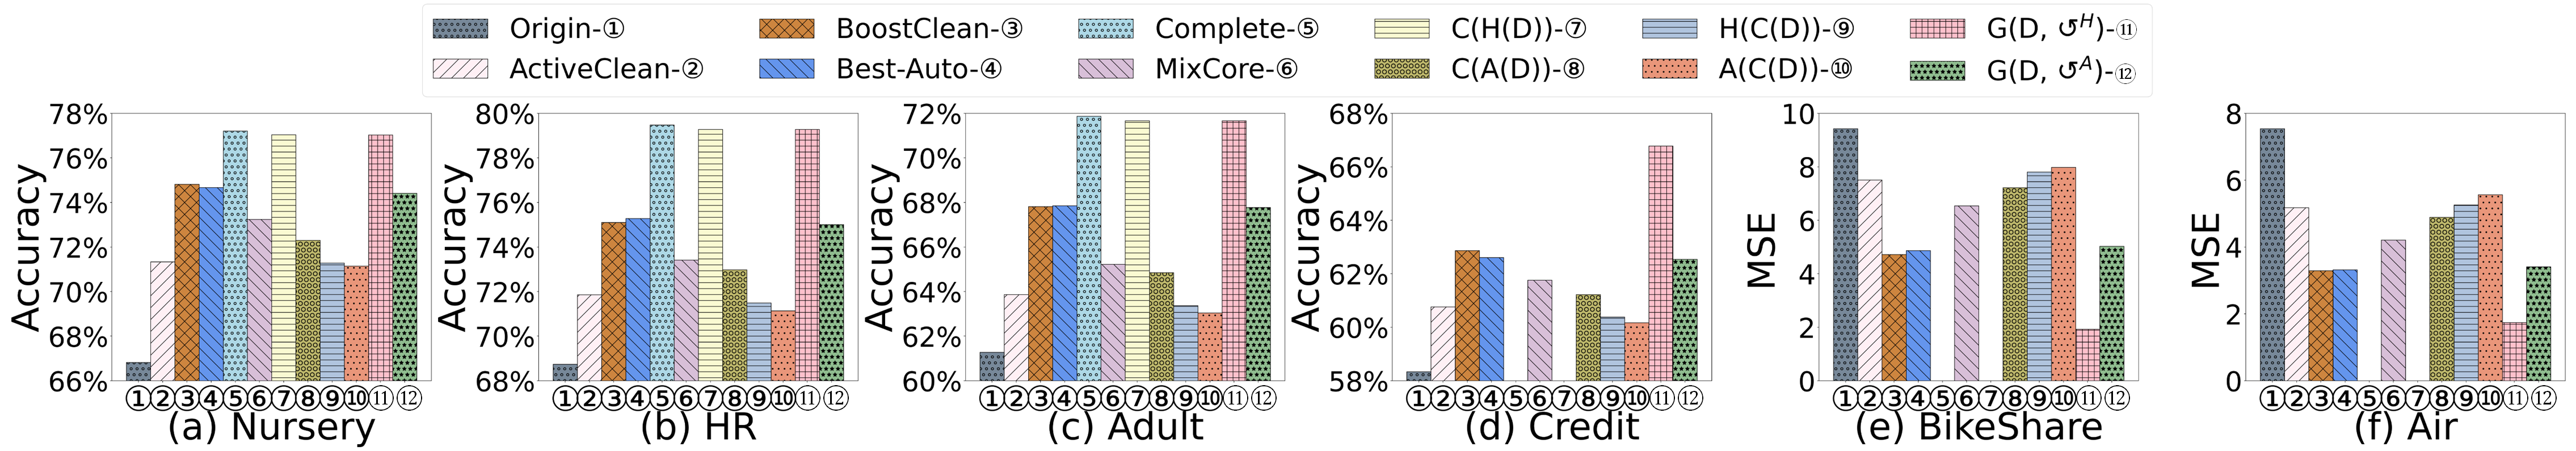
\includegraphics[width=\textwidth]{figs/effectiveness_new.png}
%	\vspace{-2.5em}
	\caption{Effectiveness of different methods.}
	\label{fig:effectiveness}
%	\vspace*{-1.2em}
\end{figure*}


%\begin{figure*}[!ht]
%	\centering
%	
\includegraphics[width=\textwidth]{figs/efficiency}
%	\vspace{-2.5em}
%	\caption{Efficiency of different methods. Note that only machine cost (i.e., runtime of machine) is considered.}
%	\label{fig:efficiency}
%	\vspace*{-1.5em}
%\end{figure*}


\begin{figure*}
	\centering
	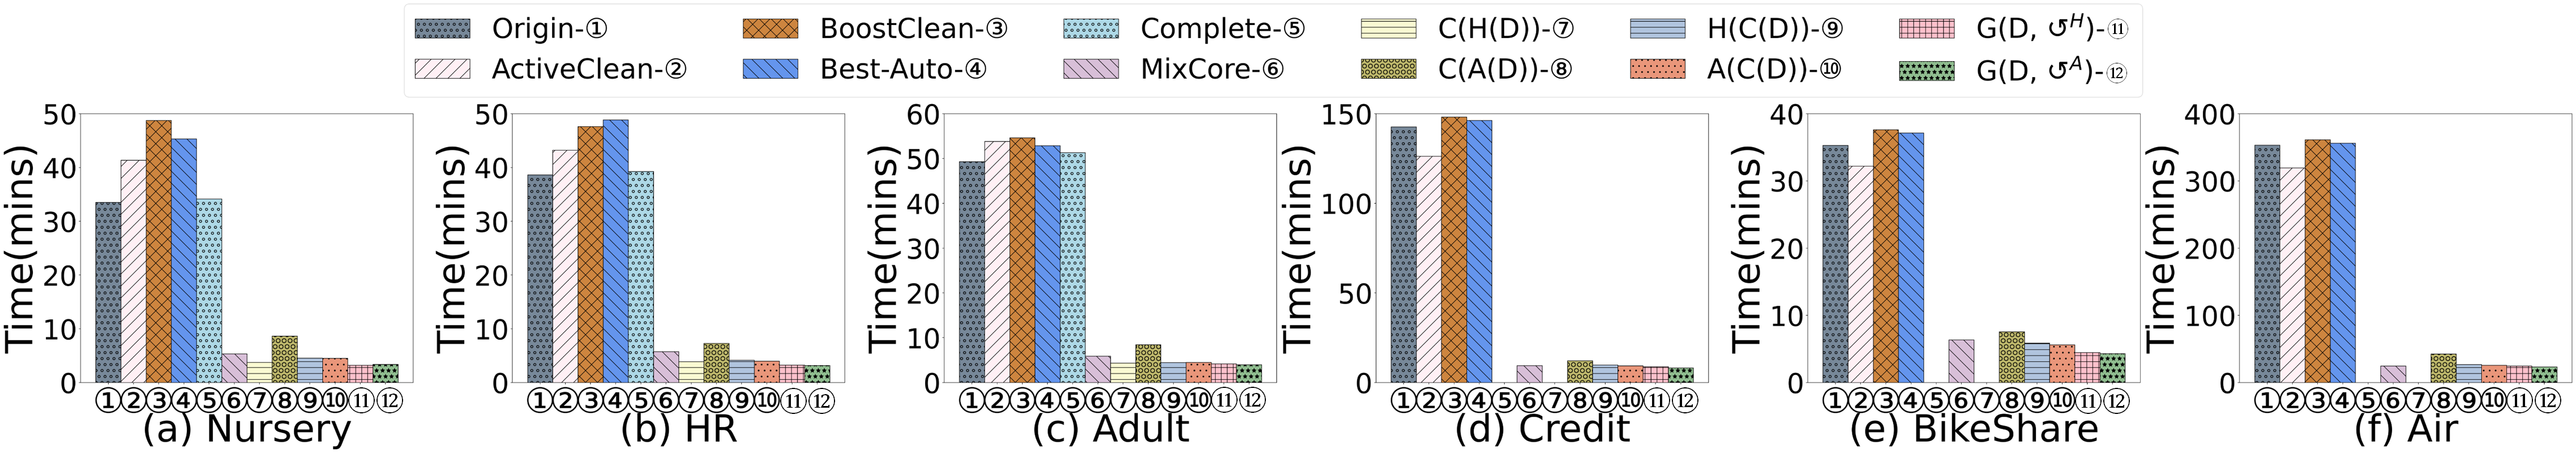
\includegraphics[width=\textwidth]{figs/efficiency_new.png}
%	\vspace{-2.5em}
	\caption{Efficiency of different methods. Note that only machine cost (i.e., runtime of machine) is considered.}
	\label{fig:efficiency}
%	\vspace*{-1.5em}
\end{figure*}



%!TEX root = ../main.tex
\subsection{Experimental Settings}

\noindent{\bf Dataset.} We evaluate on 6 real-world datasets that are often used in the field of data imputation~\cite{DBLP:conf/icde/LiRBZCZ21, liu2021adaptive, DBLP:journals/pvldb/KrishnanWWFG16,DBLP:journals/pvldb/KarlasLWGC0020}, as shown in Table~\ref{tbl:dataset}, where $M$ denotes the number of attributes.   
%They cover different downstream ML tasks, including binary classification, multi-classification and regression.  

%Among these datasets, there are not enough missing values in the some of them. Thus, we manually create some incomplete tuples for them. We can also obtain the ground truth of these manually created missing values to better compare different baselines. 
%In addition, numerical attribute is hard to impute, thus, we convert them to categorical attribute using bucketing technique. The details of these datasets are as below.

\noindent{\bf (1) \nursery}~\cite{nursery} is a multi-classification task, which  predicts ``{\it the level of recommendation for whether a child goes to school}''. There are five different levels, \ie $\{ {\tt not\_recom, priority, recommend, spec\_prior, very\_recom} \}$. %There are 9 categorical attributes. %The size of train, validation and test are 10960, 1000 and 1000. We manually created 3000 incomplete tuples in the train dataset.
{\bf (2) \hr}~\cite{chai2022selective} is a binary classification task of ``{\it predicting whether an employee would change the job}''.  %There are 12 attributes, one of which  is numerical. %and we convert it to categorical attribute using bucketing technique. The size of train, validation and test data are 18287, 2000 and 2000. In the train dataset, there are 5000 incomplete tuples.
{\bf (3) \adult}~\cite{adult} is a binary classification task that predicts ``{\it if the annual revenue of a people is over 50000 dollars}''. %There are 14 attributes in this dataset, 6 of which are categorical. %The size of train, validation and test dataset are 32842, 8000 and 8000. In the train dataset, there are 12500 incomplete tuples. 
{\bf (4) \credit}~\cite{kaggle} is a binary classification task that predicts ``{\it whether the loan will be deferred based on a person's economic situation}''.  %The size of train, validation and test dataset are 131,000, 4000 and 4000. In the train dataset, there are 87000 incomplete tuples.
{\bf (5) \bike}~\cite{bike} is a regression task that predicts ``{\it the number of bike sharing in a given time}''. %There are 15 attributes in this dataset, 5 of which are numerical data. %The size of train, validation and test dataset are 13300, 2000 and 2000. In the train dataset, there are 5100 incomplete tuples.
{\bf (6) \air}~\cite{auctus} is a regression task that predicts ``{\it the air quality at a certain time}''. %There are 18 attributes in this dataset, 12 of which are numerical data.
{\bf (7) \imdb}~\cite{DBLP:journals/pvldb/LeisGMBK015} refers to a dataset that \textit{predicts the rating (1-10) of movies}, which contains the basic information of movies, \eg \texttt{movie\_id, title, production\_year}.
%
{\bf (8) \imdbl}~\cite{DBLP:journals/pvldb/LeisGMBK015} is the large vision of \imdb, which contains 4,000,000 records with the same attributes.

%Table~\ref{xxx} shows the statistics of these datasets.

For datasets (1)-(3) and (7)-(8), we follow existing works~\cite{DBLP:journals/jbd/KhanH20,DBLP:conf/icml/YoonJS18,DBLP:conf/mlsys/WuZIR20} to manually inject missing values until the  rate of missing tuples is 30\%, and we will vary the percentage of incomplete tuples in Section~\ref{exp:sec:sensitivity}. Datasets (4)-(6) already contain missing values. For all datasets, we randomly split them for 80\%/10\%/10\% as train/validation/test sets.






\noindent{\bf Evaluation metrics.}
We mainly evaluate the effectiveness and efficiency of \ours and  baselines. For effectiveness, we use the {\it prediction accuracy} for the classification task and use the {\it mean square error} ($MSE = \frac{\sum_{i=1}^N(y_i-\hat{y}_i)}{N}$, where $N$ denotes the size of test set) for the regression task. 

For efficiency, we focus on the machine cost (\ie the runtime of machine) as well as the human cost (the number of tuples imputed by human for human-involved methods). For datasets (1)-(3) and (7)-(8), we have the ground truth of missing tuples, so we use them to simulate the human imputation. For datasets (4)-(6), we leverage the expert to impute missing values in the coreset by looking at the top-5 values recommended by the automatic method as a reference. Note that we only involve humans when it is affordable. For baselines that require humans to impute a lot of missing tuples (\ie~\truth~and $\one$ as below), we will not apply them on datasets (4)-(6).

\noindent{\bf Baselines.} We compare \ours and \ours$^+$ with a variety of baselines.

%\noindent{\bf (1) \noclean} refers to just training on $\train$. \cc{necessary?}



%\noindent{\bf (3) \truthcore} first uses the ground truth to impute the missing values and then selects the coreset for the cleaned dataset. Similar to \truth, it only works for the datasets with manually created missing values. 

%\noindent{\bf (3) \mice} is a typical missing value imputation approach. \mice uses linear regression to estimate the missing values. \mice conducts imputation for a missing value several times and uses the average value as the final result.

%\noindent{\bf (5) \missf} is a tree-based imputation method. It recasts data imputation as a prediction task and uses random forest to predict the missing values.

%Data are imputed by regressing each variable in turn against all other variables and then predicting missing data for the dependent variable using the fitted forest.
\begin{table}
	\centering
	\caption{Statistics of datasets}
	\vspace{-1em}
	{\small
	\begin{tabular}{ccccc}
		\hline
		{\bf Dataset} & {\bf $|\train|$} & {\bf $m$} & {\bf $\#$ Incomp. Tuples} & {\bf Task}\\
		\hline	
		\nursery & 	10960 & 9 & 3218 & Multi-Class. \\
		\hr & 18287 & 12 & 5475 & Binary Class. \\
		\adult & 32842 & 14 & 10752 & Binary Class. \\
		\credit & 131,000 & 11 & 76813 & Binary Class. \\
		\bike & 13300 & 15 & 4821 & Regression \\
		\air & 437,200  & 18 & 128,372 & Regression\\
		\imdb & 1,000,000 & 40 & 331,189 & Multi-Class.\\
		\imdbl & 4,000,000 & 40 & 1,312,908 & Multi-Class.\\
		\hline
	\end{tabular}
	}
	\label{tbl:dataset}
%	\vspace{-1.8em}
\end{table}

\noindent{\bf (1) \noclean}~refers to just training on $\train$.

\noindent{\bf (2) \actclean}~\cite{DBLP:journals/pvldb/KrishnanWWFG16} is an iterative data cleaning framework, which estimates the impact of tuples  and prioritizes cleaning the tuples that much affect the model performance. In each iteration, it can ask the human to clean a sample subset of tuples. We set the sample size to 50, same as the paper. 

\noindent{\bf (3) \boostclean}~\cite{DBLP:journals/corr/abs-1711-01299} is an automatic  data cleaning method that iteratively selects a cleaning method from several pre-defined algorithms, applies to the train dataset and  updates the model.  We use MICE~\cite{royston2011multiple}, MISSForest~\cite{DBLP:journals/bioinformatics/StekhovenB12}, GAIN~\cite{DBLP:conf/icml/YoonJS18} as pre-defined algorithms.


\noindent{\bf (4) \gain}  uses MICE~\cite{royston2011multiple}, MISSForest~\cite{DBLP:journals/bioinformatics/StekhovenB12}, GAIN~\cite{DBLP:conf/icml/YoonJS18} to respectively impute the train set and selects the one that achieves the highest accuracy on the validation set.

\noindent{\bf (5) \truth} is an ideal case that trains on the ground truth, \ie $\trainc$. Note that only datasets (1)-(3) have the ground truth to evaluate this baseline.  Datasets (4)-(6) do not have the ground truth and it is  too expensive to ask the human to impute so many missing values.

\noindent{\bf (6) \mixcore} is a baseline that selects a coreset from all complete tuples, and then we randomly select some incomplete tuples to impute. We set the number of incomplete tuples to be imputed equal to that of  other baselines for fair comparison. Finally we train with the tuples in the coreset plus the  imputed ones.



%It treats the data cleaning as a minimax optimization problem. The generator is optimized to impute the incomplete tuples and makes them as similar as possible to the complete tuples. While the discriminator is utilized to distinguish the imputed tuples. Thus, the incomplete tuples can be imputed during this minimax game.

%\noindent{\bf (7) \rand} randomly samples a subset from the dirty dataset $\train$ and imputes the missing values in it. Then, it trains a downstream model on this subset.


\noindent{\bf (7) $\one$} first involves human to impute the dataset $\train$ and then selects a coreset. Similar to \truth, only datasets (1)-(3) can be evaluated on it because they have the ground truth. The coreset selection solution is the algorithm in~\cite{DBLP:conf/icml/MirzasoleimanBL20}, which is a greedy algorithm by modifying Algorithm 1 without considering the possible worlds.


\noindent{\bf (8)  $\two$} first uses automatic data imputation methods to impute the dataset $\train$, and then selects a coreset using the same method of baseline (7).

\noindent{\bf (9) $\three$} directly selects a coreset based on $\train$ and then asks human to impute the incomplete tuples of the coreset.

\noindent{\bf (10) $\four$} also directly selects a coreset from $\train$, it then uses MICE~\cite{royston2011multiple} to impute the incomplete tuples in the coreset.

\noindent{\bf Our solutions.} We compare \ours and its variants.

\noindent{\bf (11) $\seven$} uses \ours to select the coreset and iteratively asks human to impute incomplete tuples (one tuple per human iteration) during the coreset selection process.

\noindent{\bf (12) $\eight$} is similar to $\goodfunc(\train,\circlearrowleft^\humanfunc)$, but the automatic  MICE  method is used.

\noindent{\bf (13) $\nine$} uses group-based method to accelerate \ours, which selects the coreset and iteratively asks human to impute incomplete tuples (one tuple per human iteration) during the coreset selection process.

\noindent{\bf (14) $\ten$} is similar to $\nine$, but the automatic  MICE  method is used.


Besides, since the coreset of $\five$ (or $\six$) is too expensive to compute due to the large number of possible worlds, we do not directly compare with it. Instead, we will limit the number of possible worlds of each tuple to 3 as discussed in Section~\ref{subsec:batch} and evaluate in Section~\ref{exp:sec:batchalgo}.

%\noindent{\bf (12) $\five$} first uses \ours to select a coreset and then involves human to impute this coreset. Since the machine cost is too high, we limit the number of possible worlds of each tuple to 3 and evaluate in Section~\ref{exp:sec:batchalgo}.

%\noindent{\bf (13) $\six$} also uses \ours to select a coreset and leverages MICE to impute this coreset. For the same reason as $\five$, we also  limit $l=3$  and evaluate in Section~\ref{exp:sec:batchalgo}.

 



%\noindent{\bf (10) \autocore} first uses an automatic data imputation method (\eg MICE) to impute the dirty dataset $\train$. Then, it selects a coreset of the cleaned dataset and involves human to review the missing values in the coreset.




\noindent{\bf Hyper-parameter setting.}
%For classification tasks, we use SVM as the default downstream model. For regression tasks, we use linear regression as the default.
We use SVM and linear regression as the default downstream model for classification and regression tasks, respectively. We vary the downstream models in Section~\ref{exp:sec:sensitivity}. For model training, we use SGD and k-inverse decay  scheduling, \ie $\alpha_k = \alpha_0 / (1+bk)$ ($\alpha_0$ and $b$ are hyper-parameters to be tuned independently for different methods).  The sample size $h$ is set to 200 as default and we vary the  size in Section~\ref{exp:sec:sensitivity}. The number of training epochs is set as 20. %\cc{
We also impute the test data using the same method that is applied to the train data before testing.
%}

\begin{figure}
	\vspace{-1em}
	\centering
	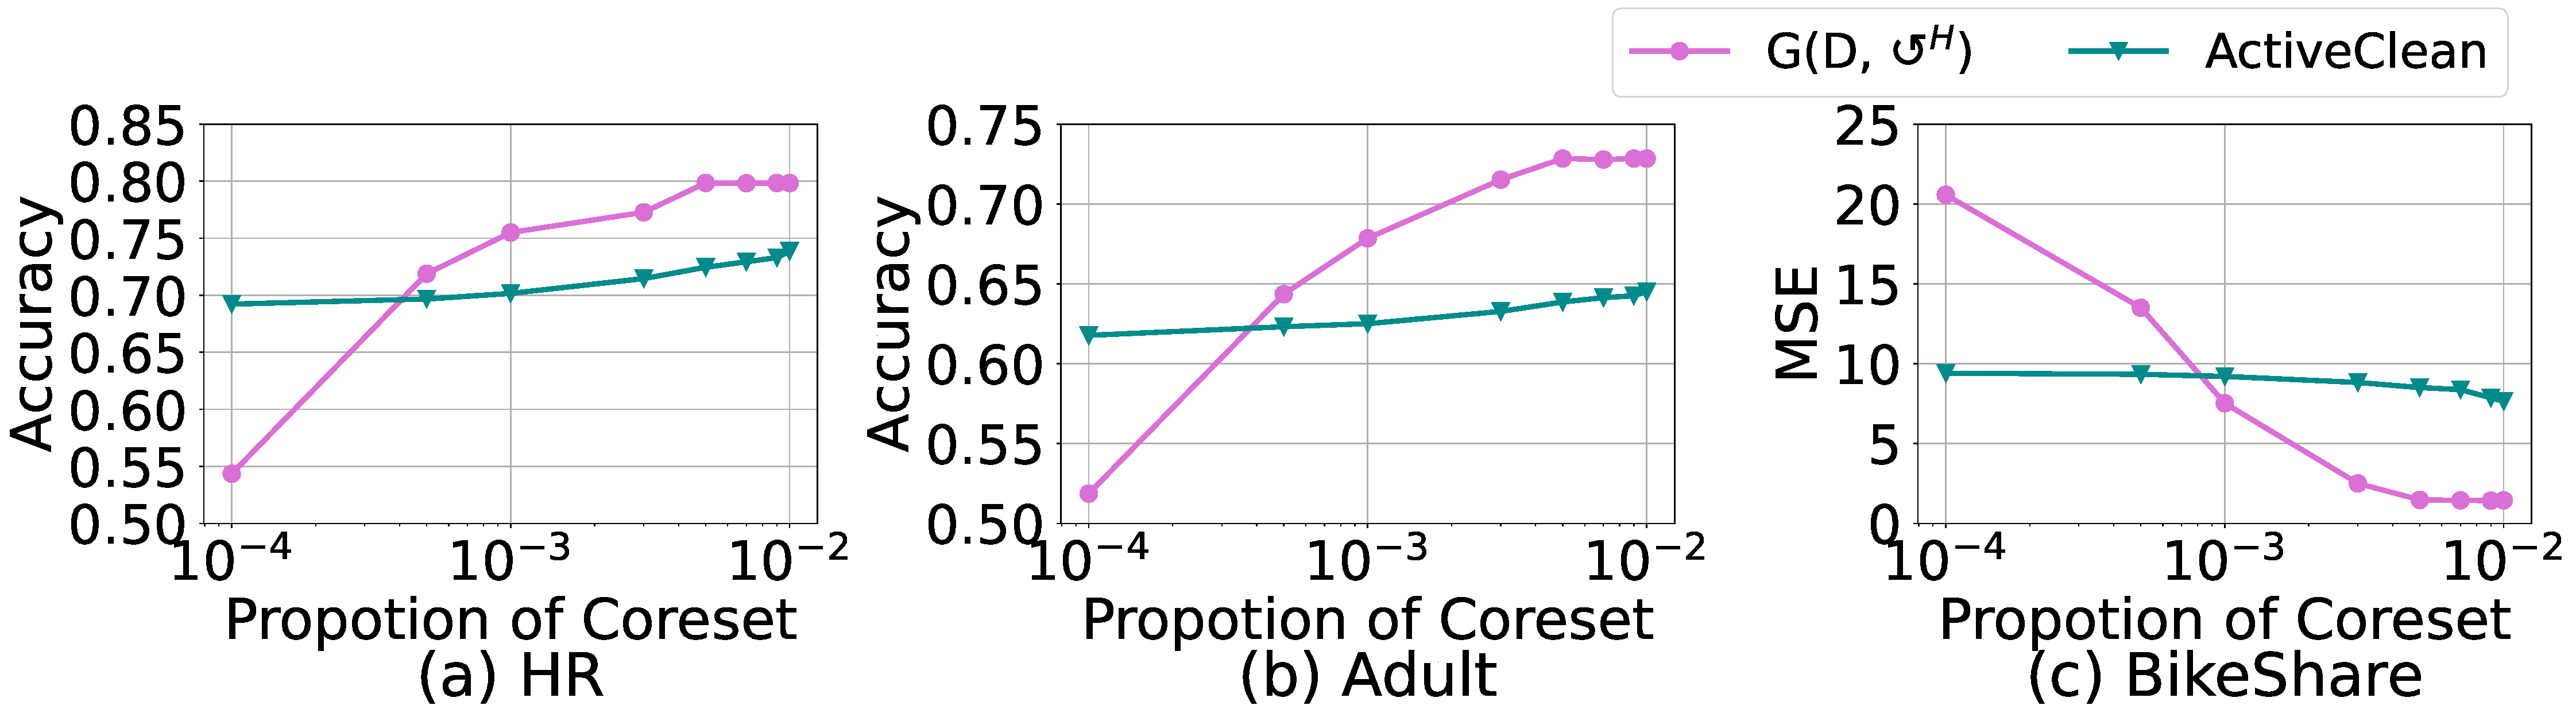
\includegraphics[width=0.6\textwidth]{figs/e2e}
%	\vspace{-2.5em}
	\caption{ Coreset size selection of \ours.}
	\label{fig:e2e}
%	\vspace{-1.8em}
\end{figure}





\begin{figure}   
	\centering
	\begin{minipage}[t]{0.32\textwidth}
		\centering
		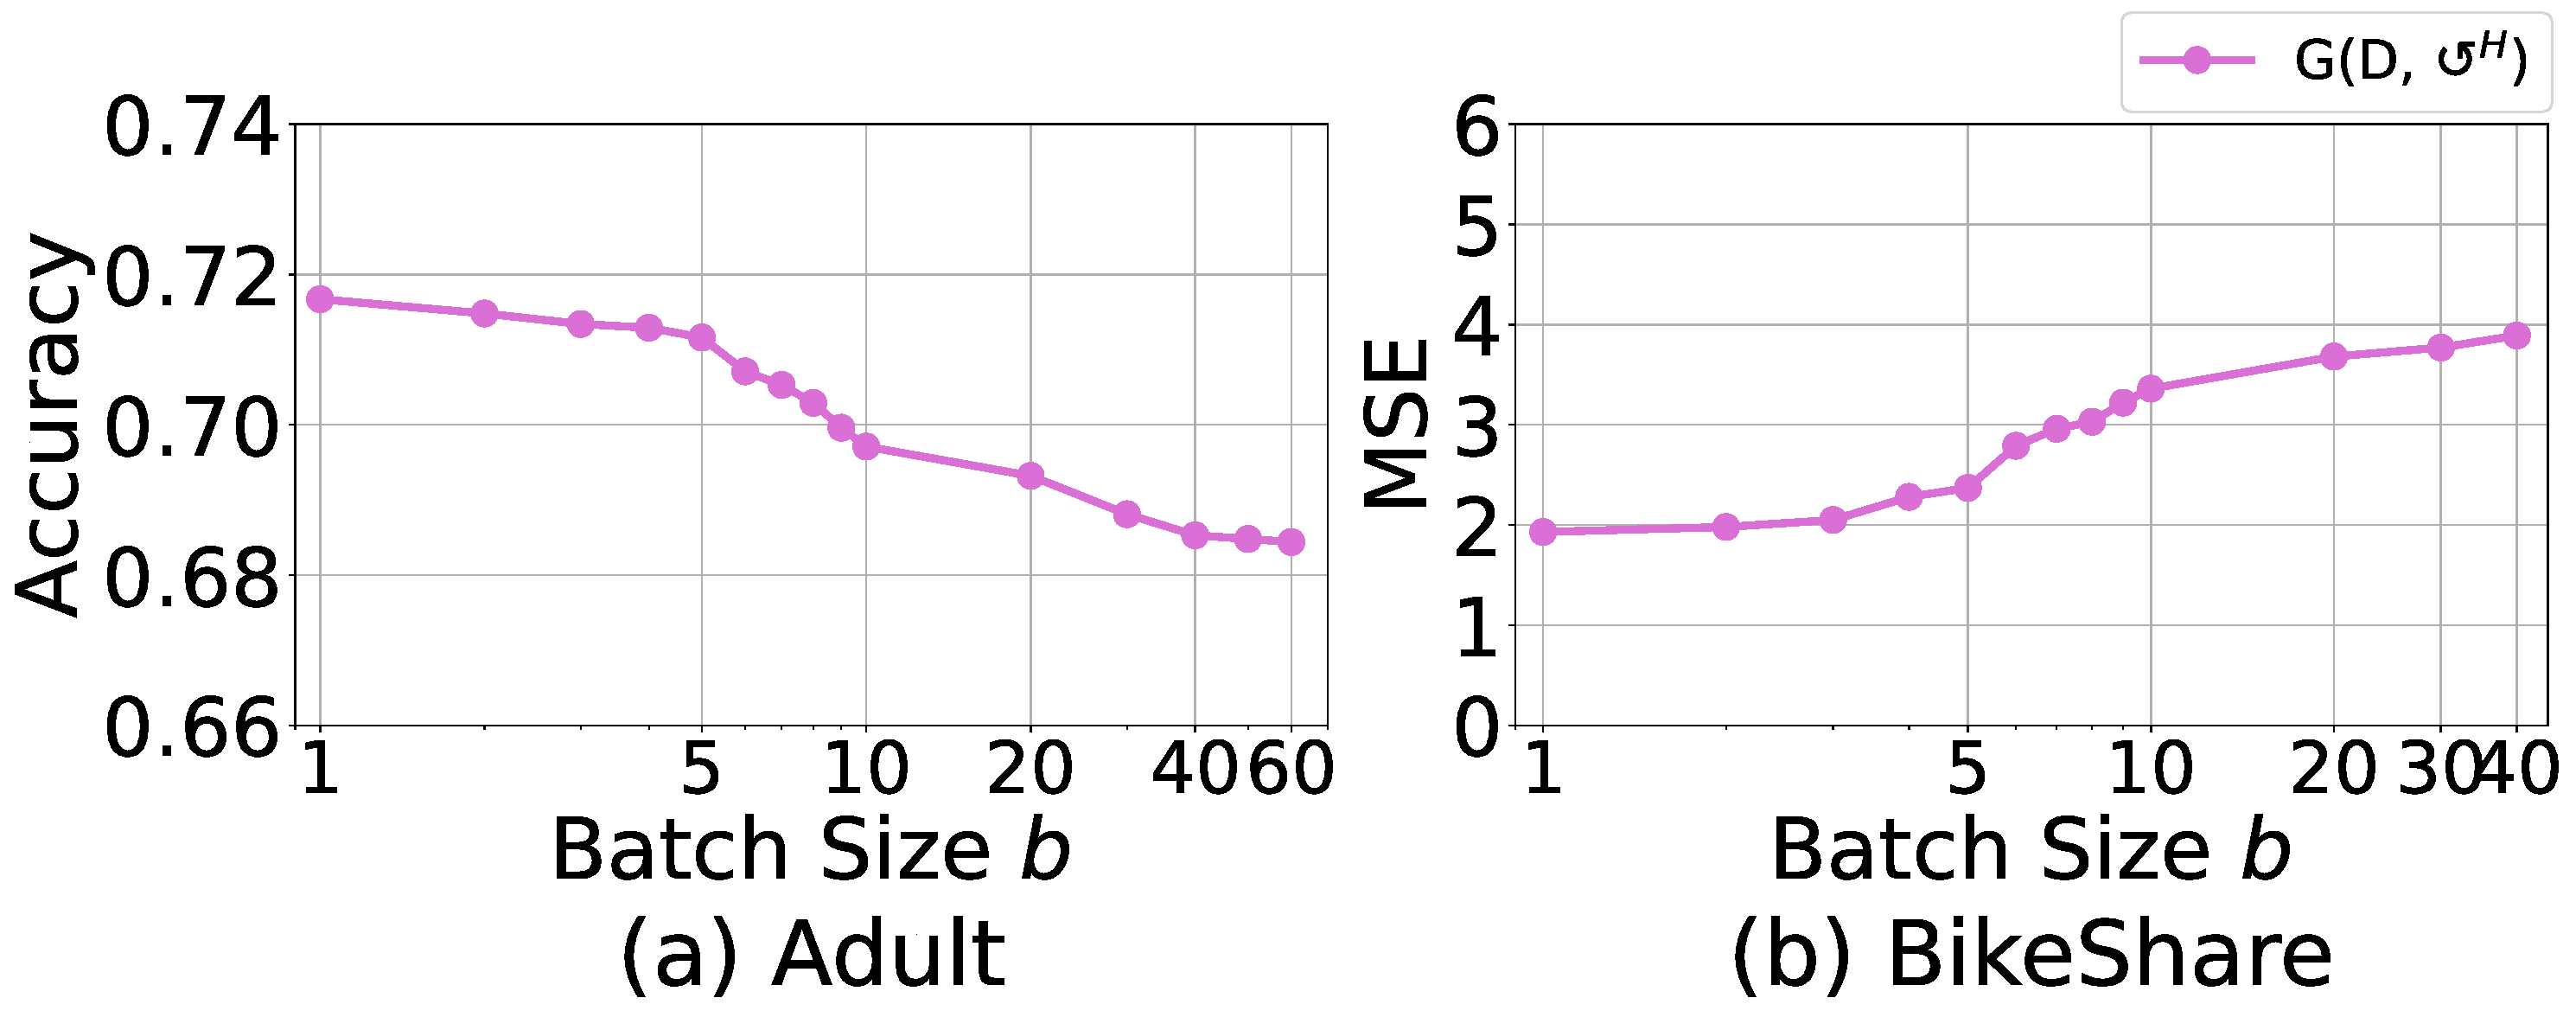
\includegraphics[width=\columnwidth]{figs/batchsize}
		\vspace{-2.5em}
		\caption{\ours for batch algorithm.}
		\label{fig:batchalg}
	\end{minipage}
	\begin{minipage}[t]{0.32\textwidth}
		\centering
		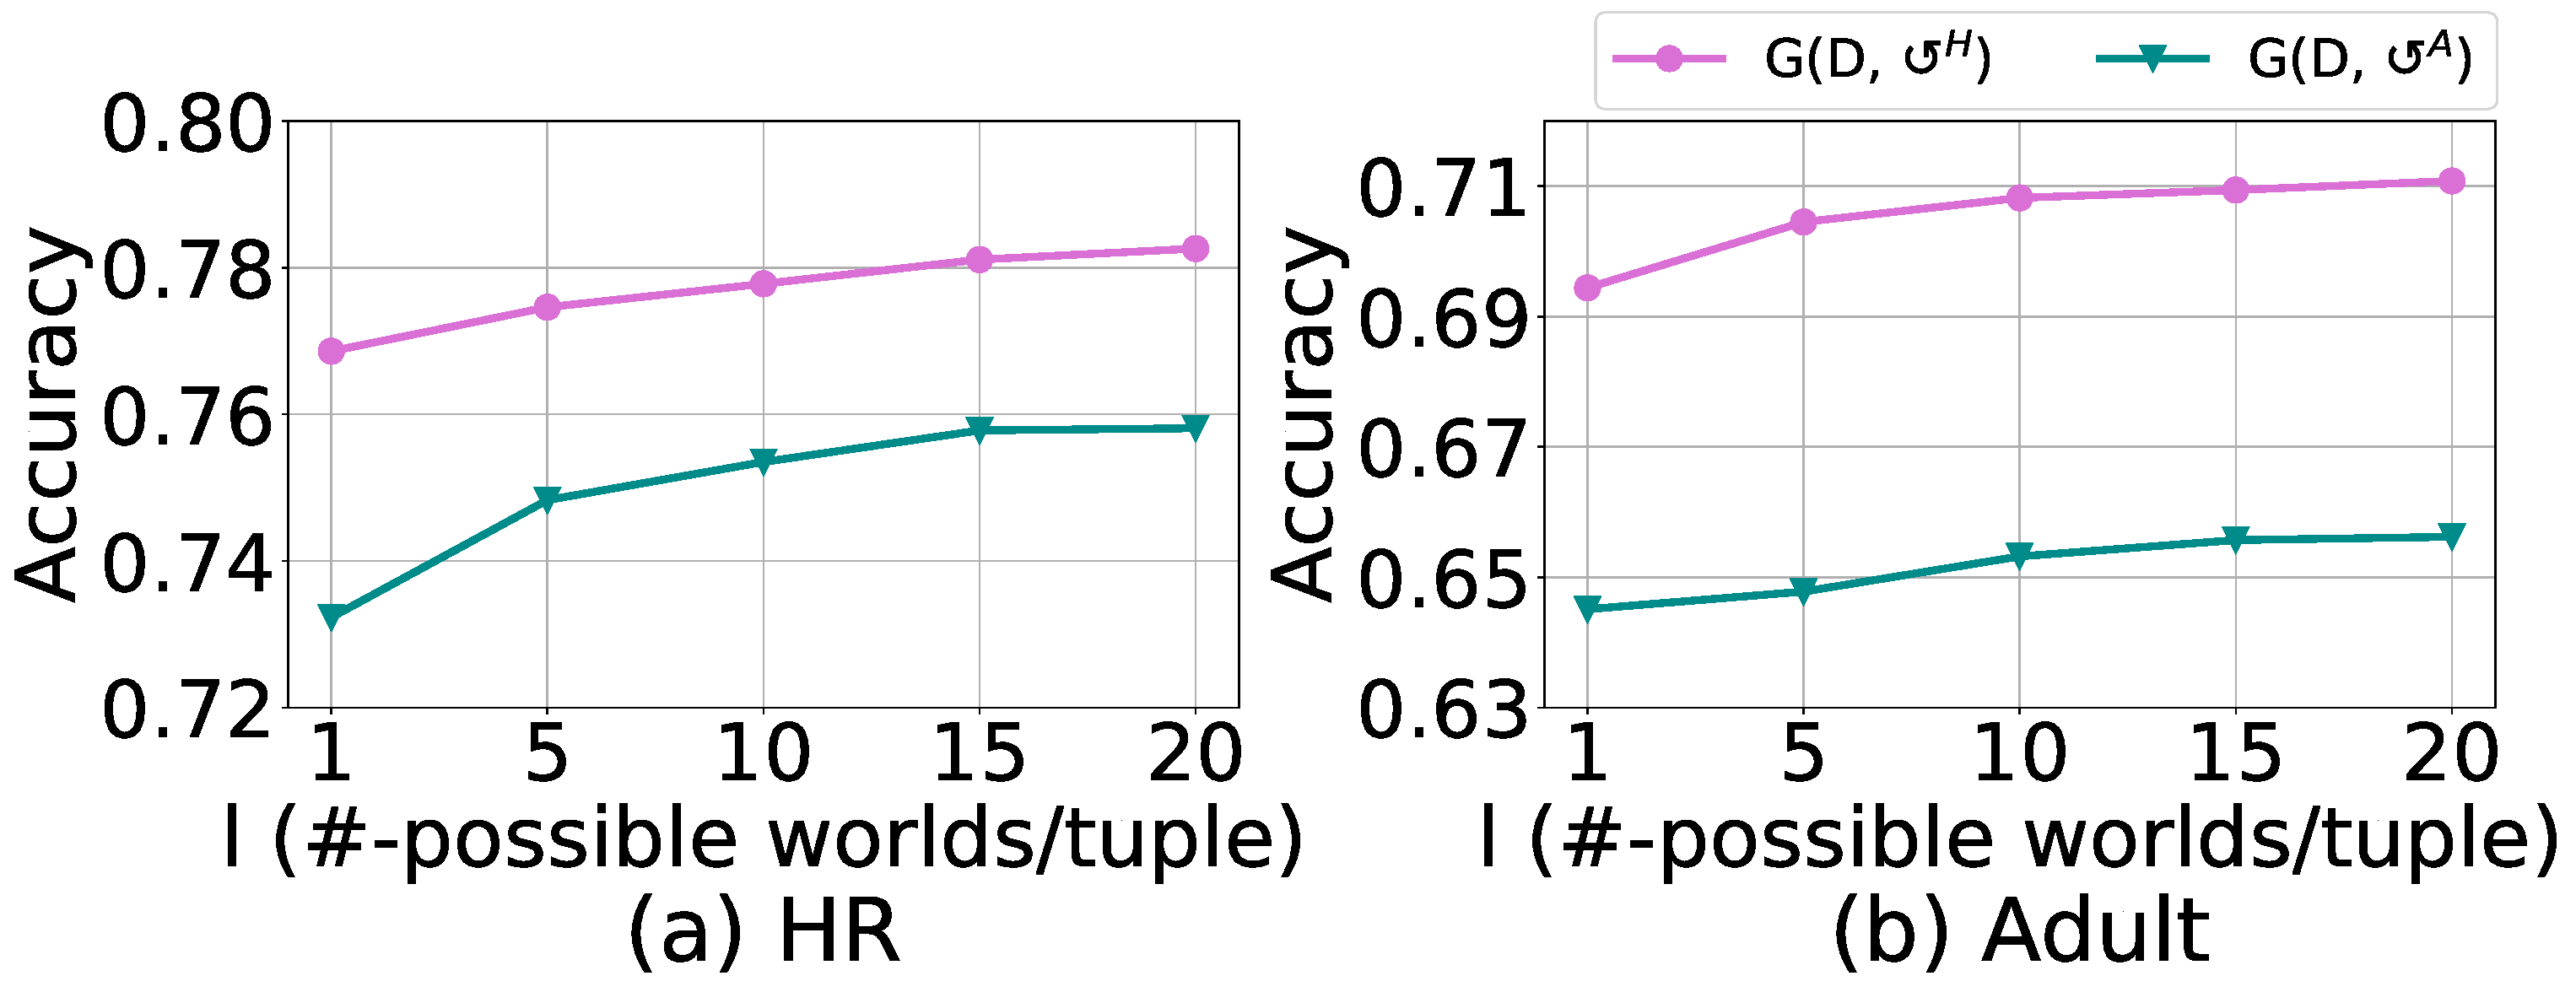
\includegraphics[width=\columnwidth]{figs/vary_l_effectiveness}
		\vspace{-2.5em}
		\caption{Effectiveness when varying $l$.}
		\label{fig:vary_l_effect}
	\end{minipage}
	\begin{minipage}[t]{0.32\textwidth}
		\centering
		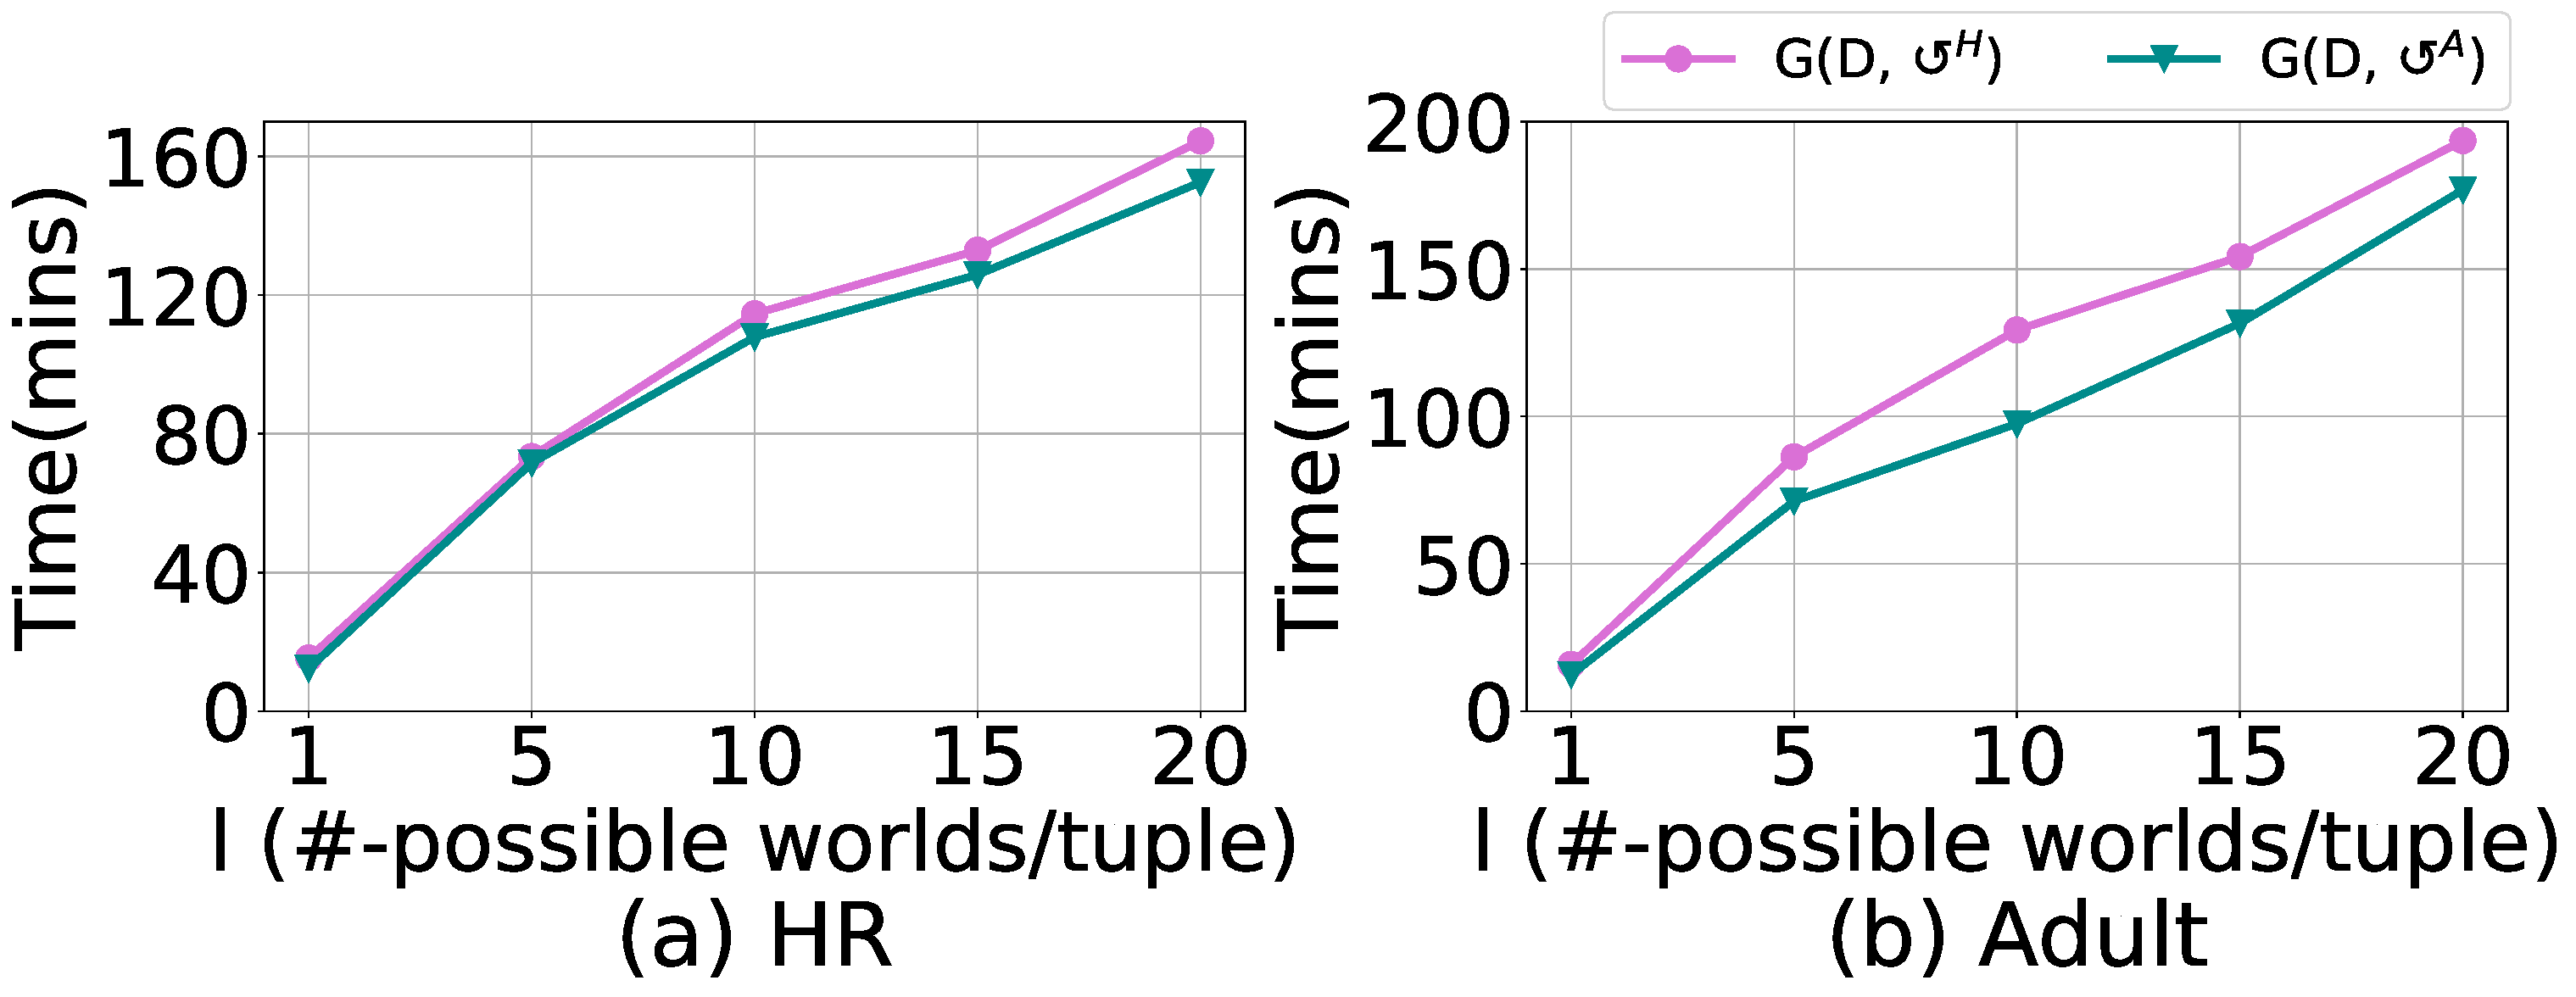
\includegraphics[width=\columnwidth]{figs/vary_l_efficiency}
		\vspace{-2.5em}
		\caption{Efficiency when varying $l$.}
		\label{fig:vary_l_efficient}
	\end{minipage}
%	\vspace*{-1.8em}   
\end{figure}





%!TEX root = ../main.tex



\subsection{Overall Evaluation}\label{exp:sec:overall}

\begin{table}
	\centering
	\caption{Human cost of different methods}
	\vspace{-1.2em}
	\small
	\begin{tabular}{ccccc}
		\hline
		Dataset & $\nine$ & $\seven$ & $\three$ & $\one$\\
		\hline
		\nursery & 35 & 37 & 22 & 3278\\
		\hr & 48 & 44 & 32 & 5475\\
		\adult & 60 & 63 & 81 & 10752\\
		\credit & 57 & 52 & 67 & -\\
		\bike & 35 & 38 & 25 & -\\
		\air & 100 & 98 & 102 & -\\
		\imdb & 215 & 220 & 230 & 331189\\
		\imdbl & 520 & 511 & 530 & 1312908 \\
		\hline
	\end{tabular}
	\label{tbl:humancost}
	\vspace{-1em}
\end{table}





In this part, we compare \ours \jks{and \ours$^+$} solutions with baselines. We use $\rho = \frac{K}{|\train|}$ to denote the proportion of coreset  to the entire train set.  %\cc{
We set  $\rho=0.005$ for datasets (1)-(4), $\rho=0.001$ for datasets (5) and  $\rho=0.0005$ for larger datasets (6)-(8).
%}
 We  will further  conduct evaluation by varying the coreset size  in Section~\ref{exp:sec:end2end}.




\subsubsection{Evaluation of model accuracy.}
The results are provided in Figure~\ref{fig:effectiveness_old} \jks{and Figure~\ref{fig:effectiveness_new}}. To summarize, the result could be generally ranked as $\seven/\one/\truth$ >  $\eight/\boostclean/\gain$ > $\two$ > $\mixcore$ > $\actclean$ > $\three/\four$ > $\noclean$.
Next, we explain the results.

In general, on all datasets, our method $\seven$, \truth~ and $\one$~   perform the best. 
 \truth~ and $\one$ achieve a high accuracy because they ask the human to impute missing values accurately, but incur a high human cost.  For example, \truth~and $\one$ achieve accuracy of 71.9\% and 71.7\% on \adult. $\seven$  is competitive with them because it selects a good coreset that can well represent the unknown ground truth via gradient approximation. In addition, we can observe that $\seven$ performs better than $\eight$ because human imputation is more accurate than automatic methods. For example, on \adult, $\seven$ has an accuracy of 71.7\%, while $\eight$ and others are below 68\%. $\eight$, \boostclean and \gain have competitive performance on accuracy. \boostclean and \gain can have a not bad performance because they impute all tuples and train on the entire dataset, but they cannot achieve efficient training (see \ref{sec:exp:efficiency}). But  we can train on the much smaller coreset generated by $\eight$ with a good accuracy, because \ours considers the possible repairs to derive the coreset  that can approximate the full gradient of the entire dataset. Given the same number of tuples to be imputed by human,  $\seven$ also outperforms \actclean because we have theoretical guarantees on the gradient approximation. 
 %For example, on dataset \adult, $\eight$ has an accuracy of 69.8\%, which is better than that of \boostclean (65.8\%), \actclean (63.9\%) and \gain (65.1\%). Our method $\eight$ outperforms \boostclean because we consider possible repairs and the gradients of tuples in our algorithm.   \actclean also considers gradients of tuples, which prioritizes imputing tuples that much influence the model gradients, but they use heuristics to estimate the influence, which is not accurate enough. \gain does not perform well because it does not much consider possible repairs and not impute the tuple considering the downstream model performance.
  For other baselines,  $\three$ and $\four$ do not perform well because they select the coreset from an incomplete dataset.  $\two$ cannot achieve a good performance because the selected coreset can not well represent the complete entire dataset, as it does not consider possible repairs as our method.  %it is hard for the automatic method to always achieve a high imputation accuracy. 
  {\mixcore} does not perform well (\eg 65.2\% on \adult) because $\seven$ and $\eight$ select a better coreset considering the full data. For \noclean, on  \adult, the model  has an accuracy of 61.3\% because of the incomplete tuples.



 



\subsubsection{Evaluation of the efficiency.}~\label{sec:exp:efficiency} We  evaluate the efficiency of all methods, including the machine cost and human cost.

\noindent{\bf Machine cost.} Machine cost is shown  in Figure~\ref{fig:efficiency_old}.  The results could be ranked as $\three/\four/\seven/\eight/\one/\mixcore < \two < \truth < \noclean < \actclean < \boostclean/\gain$. We can observe that the first 5 methods in the ranking have low machine cost, mainly because they train based on the selected coreset and do not need iterative training. $\seven$ and  $\eight$ are slightly slower  because they need to iterate several possible repairs during the process of coreset selection.  But $\seven$ is still more efficient than \noclean, \truth, \boostclean and \gain by more than one order of magnitude,  because they need to train on the entire training data. 
 Moreover, \actclean~  and \boostclean are  not efficient either because they incorporate multiple training times, so as to estimate the gradient while data imputation. \gain is slow because training multiple imputation models takes time.


\noindent{\bf Human cost.} In terms of the human cost, $\one$, $\three$, $\seven$ and  \actclean~ involve human. As shown in~Table~\ref{tbl:humancost}, $\one$ is very expensive because it asks the human to impute all missing tuples. For example, on datset \adult, 10752 tuples have to be imputed. We do not compare \credit, \bike and \air for $\one$ because they do not have the ground truth.
 But $\three$ and $\seven$ are cost-effective because human just needs to impute missing tuples in the much smaller coreset. For example, they only cost 81 and 63 tuples on dataset \adult respectively. 
\actclean~ asks the human to iteratively impute the data. Given the same number of tuples to impute, our method can achieve much higher accuracy. We will  evaluate it in details in next subsection.
 



\noindent \textbf{Summary.} 
Based on the results, we have the following conclusions.
(1) Our proposed methods $\seven$ and $\eight$ can achieve high model accuracy because the selected coreset can well represent the underlying ground truth by gradient approximation considering possible repairs. Meanwhile, they are practical because of the low machine cost. (2) Compared with $\one$ that involves human to impute the entire dataset $D$, the human cost of $\seven$ is much lower, as observed in Table~\ref{tbl:humancost}, e.g., $37$ vs. $3278$ on the \nursery dataset. Thus, we can choose $\seven$ when we want to achieve high model accuracy and afford a certain human cost. (3) 
%Meanwhile, they are practical because of the low machine cost. Although $\seven$ needs human involvement, the human cost is also low. We can choose it when we want to achieve high model accuracy. 
If we neither care very much about the accuracy nor consider to incur human cost, the much more efficient $\eight$ is a good choice.





%\begin{figure}
%	\centering
%	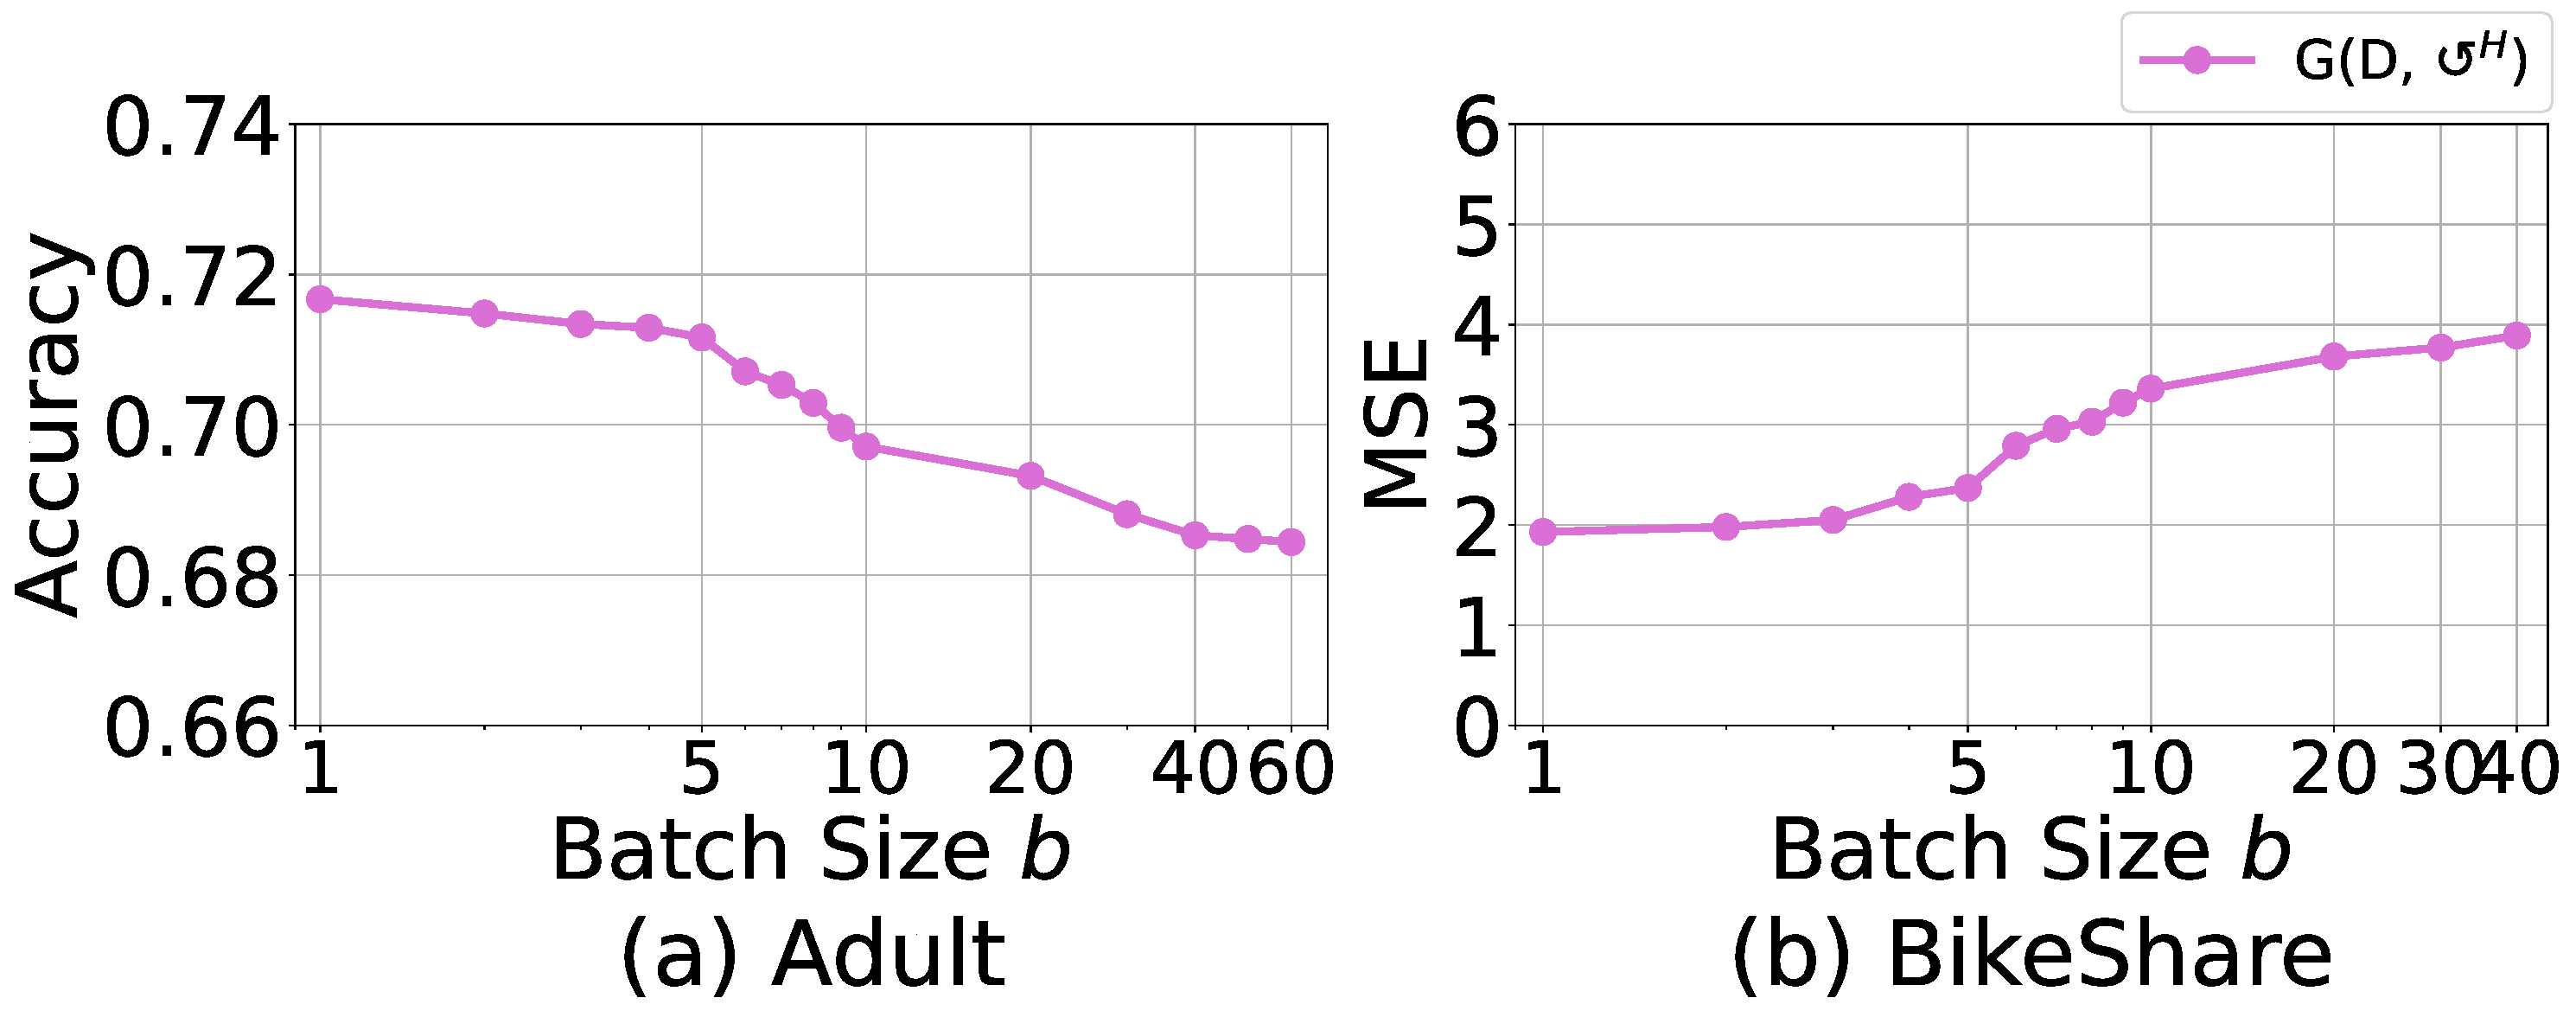
\includegraphics[width=0.7\columnwidth]{figs/batchsize}
%	\vspace{-1.5em}
%	\caption{\ours for batch algorithm.}
%	\label{fig:batchalg}
%	\vspace{-2em}
%\end{figure}



%!TEX root = ../main.tex
\vspace{-0.5em}
\subsection{Coreset Size Selection of \ours}
\label{exp:sec:end2end}



Recap that \ours needs the user-specified coreset size as input. Thus, we discuss how to select an appropriate coreset size. We adopt a simple yet effective solution that starts from a coreset with a small size, train over it and
evaluate via a validation set, enlarge the coreset and iteratively
train  until the performance does not improve much. 
To be specific, initially, we begin with $\rho = 10^{-4}$, and   enlarge the coreset by 2 times iteratively. If the performance on validation set varies no more than 0.5\% within three
successive iterations, we will
stop.
 Figure~\ref{fig:e2e} shows the performance on dataset \hr, \adult and \bike when varying the coreset size. We can see that the performance first improves rapidly, then remains  stable just after several iterations. For example, on dataset \adult, when $\rho=5\times 10^{-3}$, the accuracy has improved  to 72.85\% on the validation set. Empirically, an ideal coreset size is between $\rho=10^{-3}$ to $10^{-2}$.
 
\noindent \textbf{Summary.} The results show that coreset size is not difficult to determine. If the user is willing to specify a coreset size like in Section~\ref{exp:sec:overall} based on the empirical finding, we can directly compute a coreset without training. If she cannot, we can also get a good coreset with just several training iterations over small coresets, which is also efficient.
 
 

\noindent{\bf Compare with \actclean.} 
Figure~\ref{fig:e2e} also reports an interesting comparison with \actclean. Specifically, 
%We also compare with  \actclean by varing corein this iterative scenario.
in \actclean, we use the coreset size $K$ as the budget, i.e., number of tuples to be imputed by human in each active cleaning iteration. 
%at each point of the x-axis in Figure~\ref{fig:e2e}, we set that \actclean asks the human to impute  the same number of tuples as us, which can be regarded as a budget. 
We can observe that at the beginning, when the coreset size is very small, \actclean is better because it trains with the entire dataset including the imputed tuples, while we train the model using only  few tuples in the coreset.
However, as with the increase of the coreset size, we can see that $\seven$ outperforms \actclean. This is because \actclean uses a heuristic method to estimate the impact of tuples to the overall gradient, which is not theoretically bounded (e.g., with gradient bounds like Coreset) and thus not accurate enough.
%without the gradient bound, which is  not accurate enough.
For $\seven$, it can achieve high accuracy with a proper coreset size, which is not large.
%Besides, recap that given a budget, \actclean needs to iteratively sample tuples to clean and train, but we do not need to train if the coreset size is specified, which is more efficient.










 


\begin{figure}
	\centering
	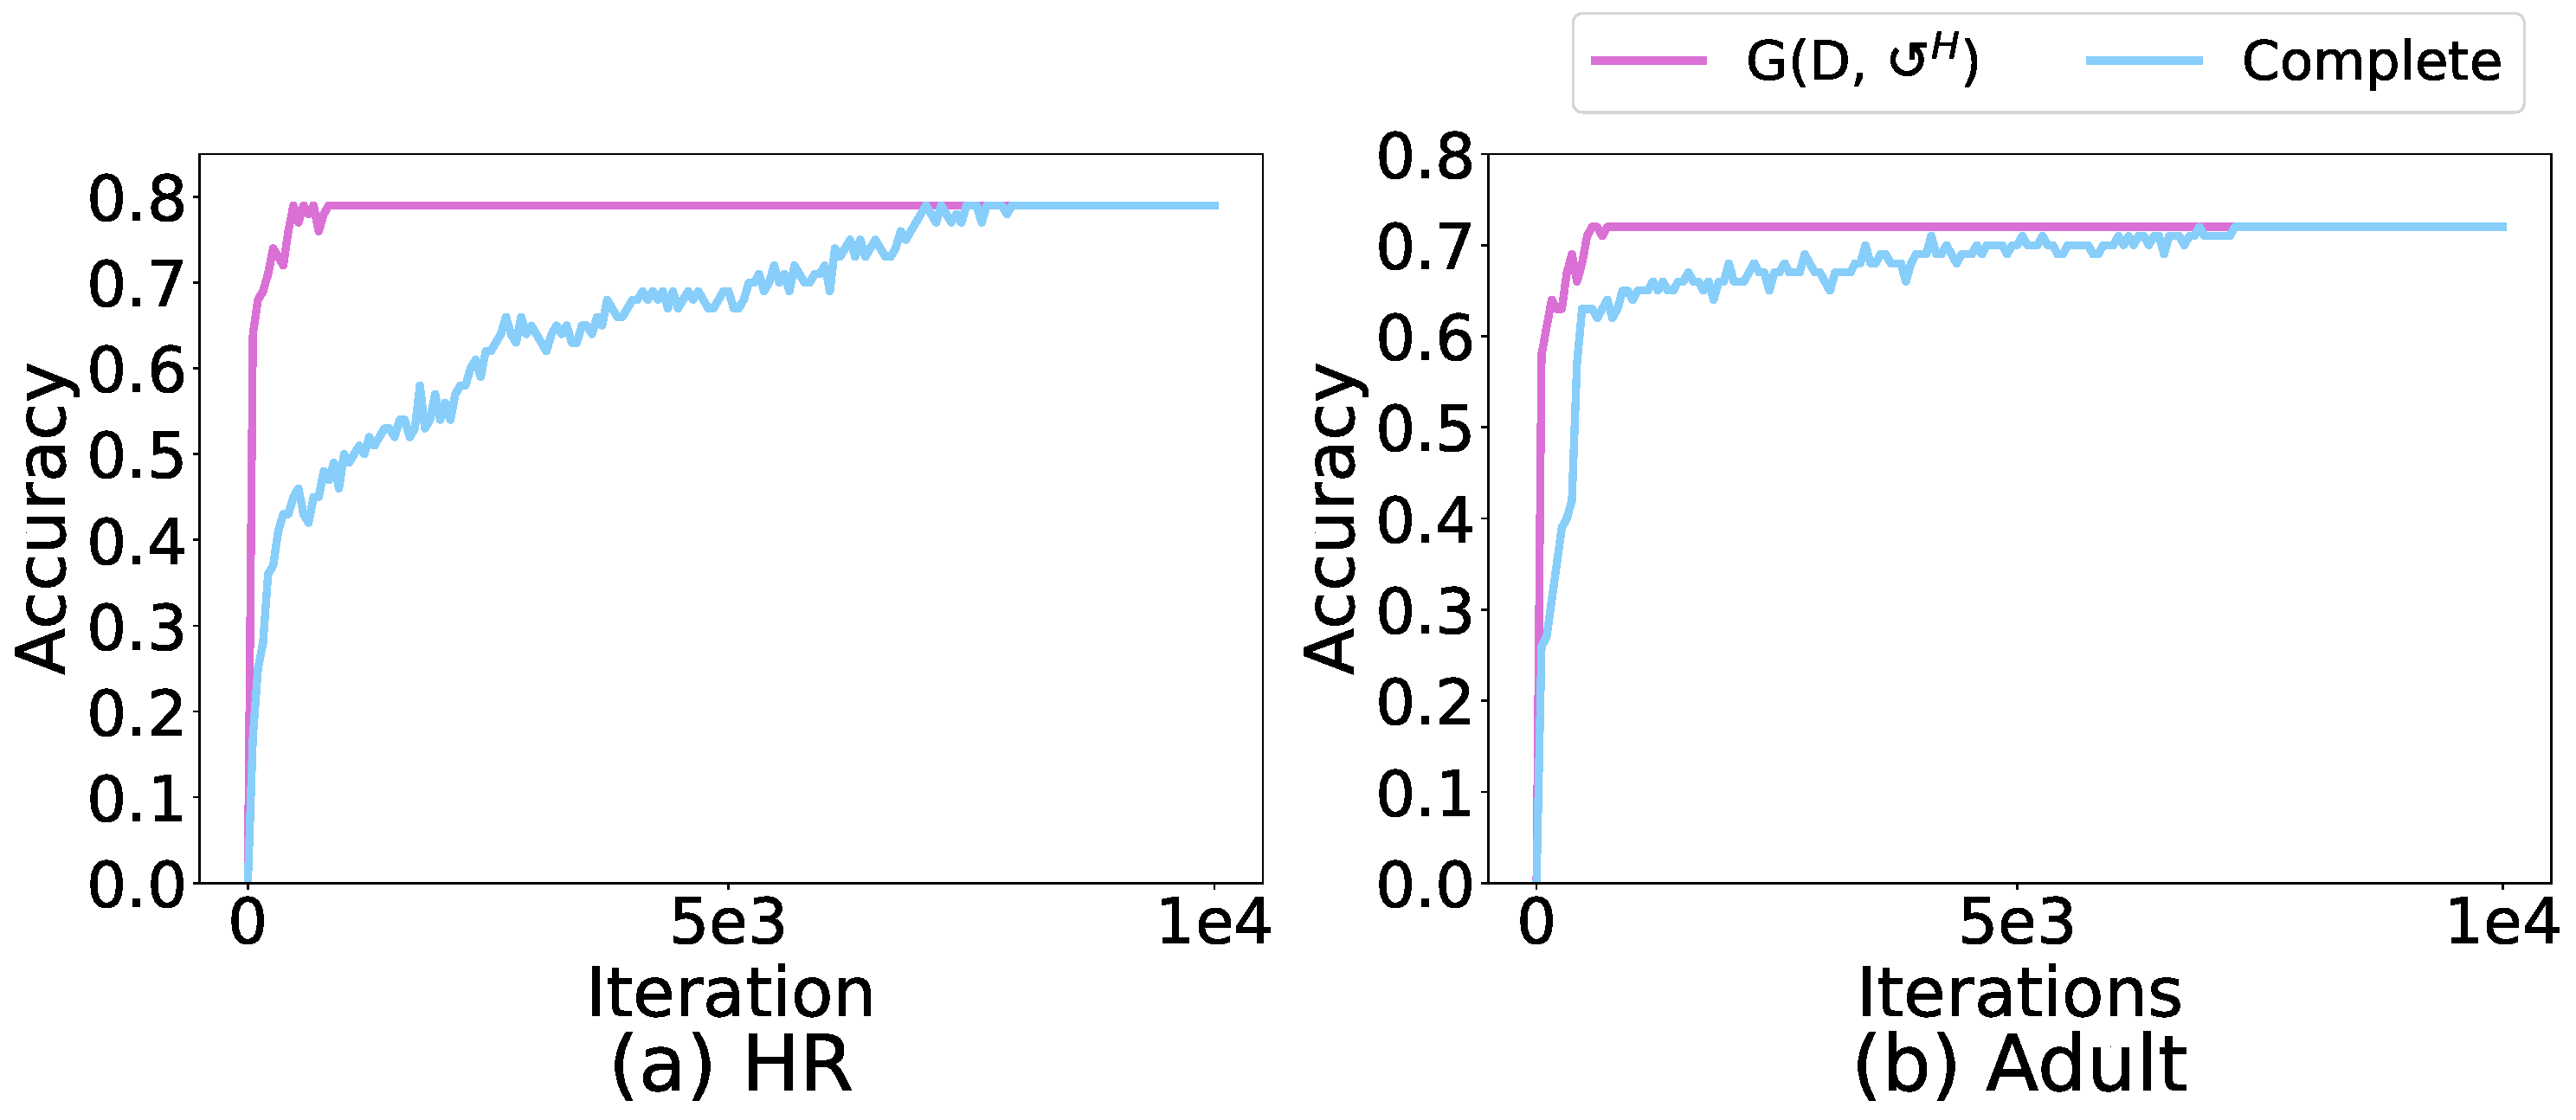
\includegraphics[width=0.5\columnwidth]{figs/converge}
%	\vspace{-1.5em}
	\caption{Convergence of \ours.}
	\label{fig:converge}
%	\vspace{-1.5em}
\end{figure}


\begin{figure}
	\centering
	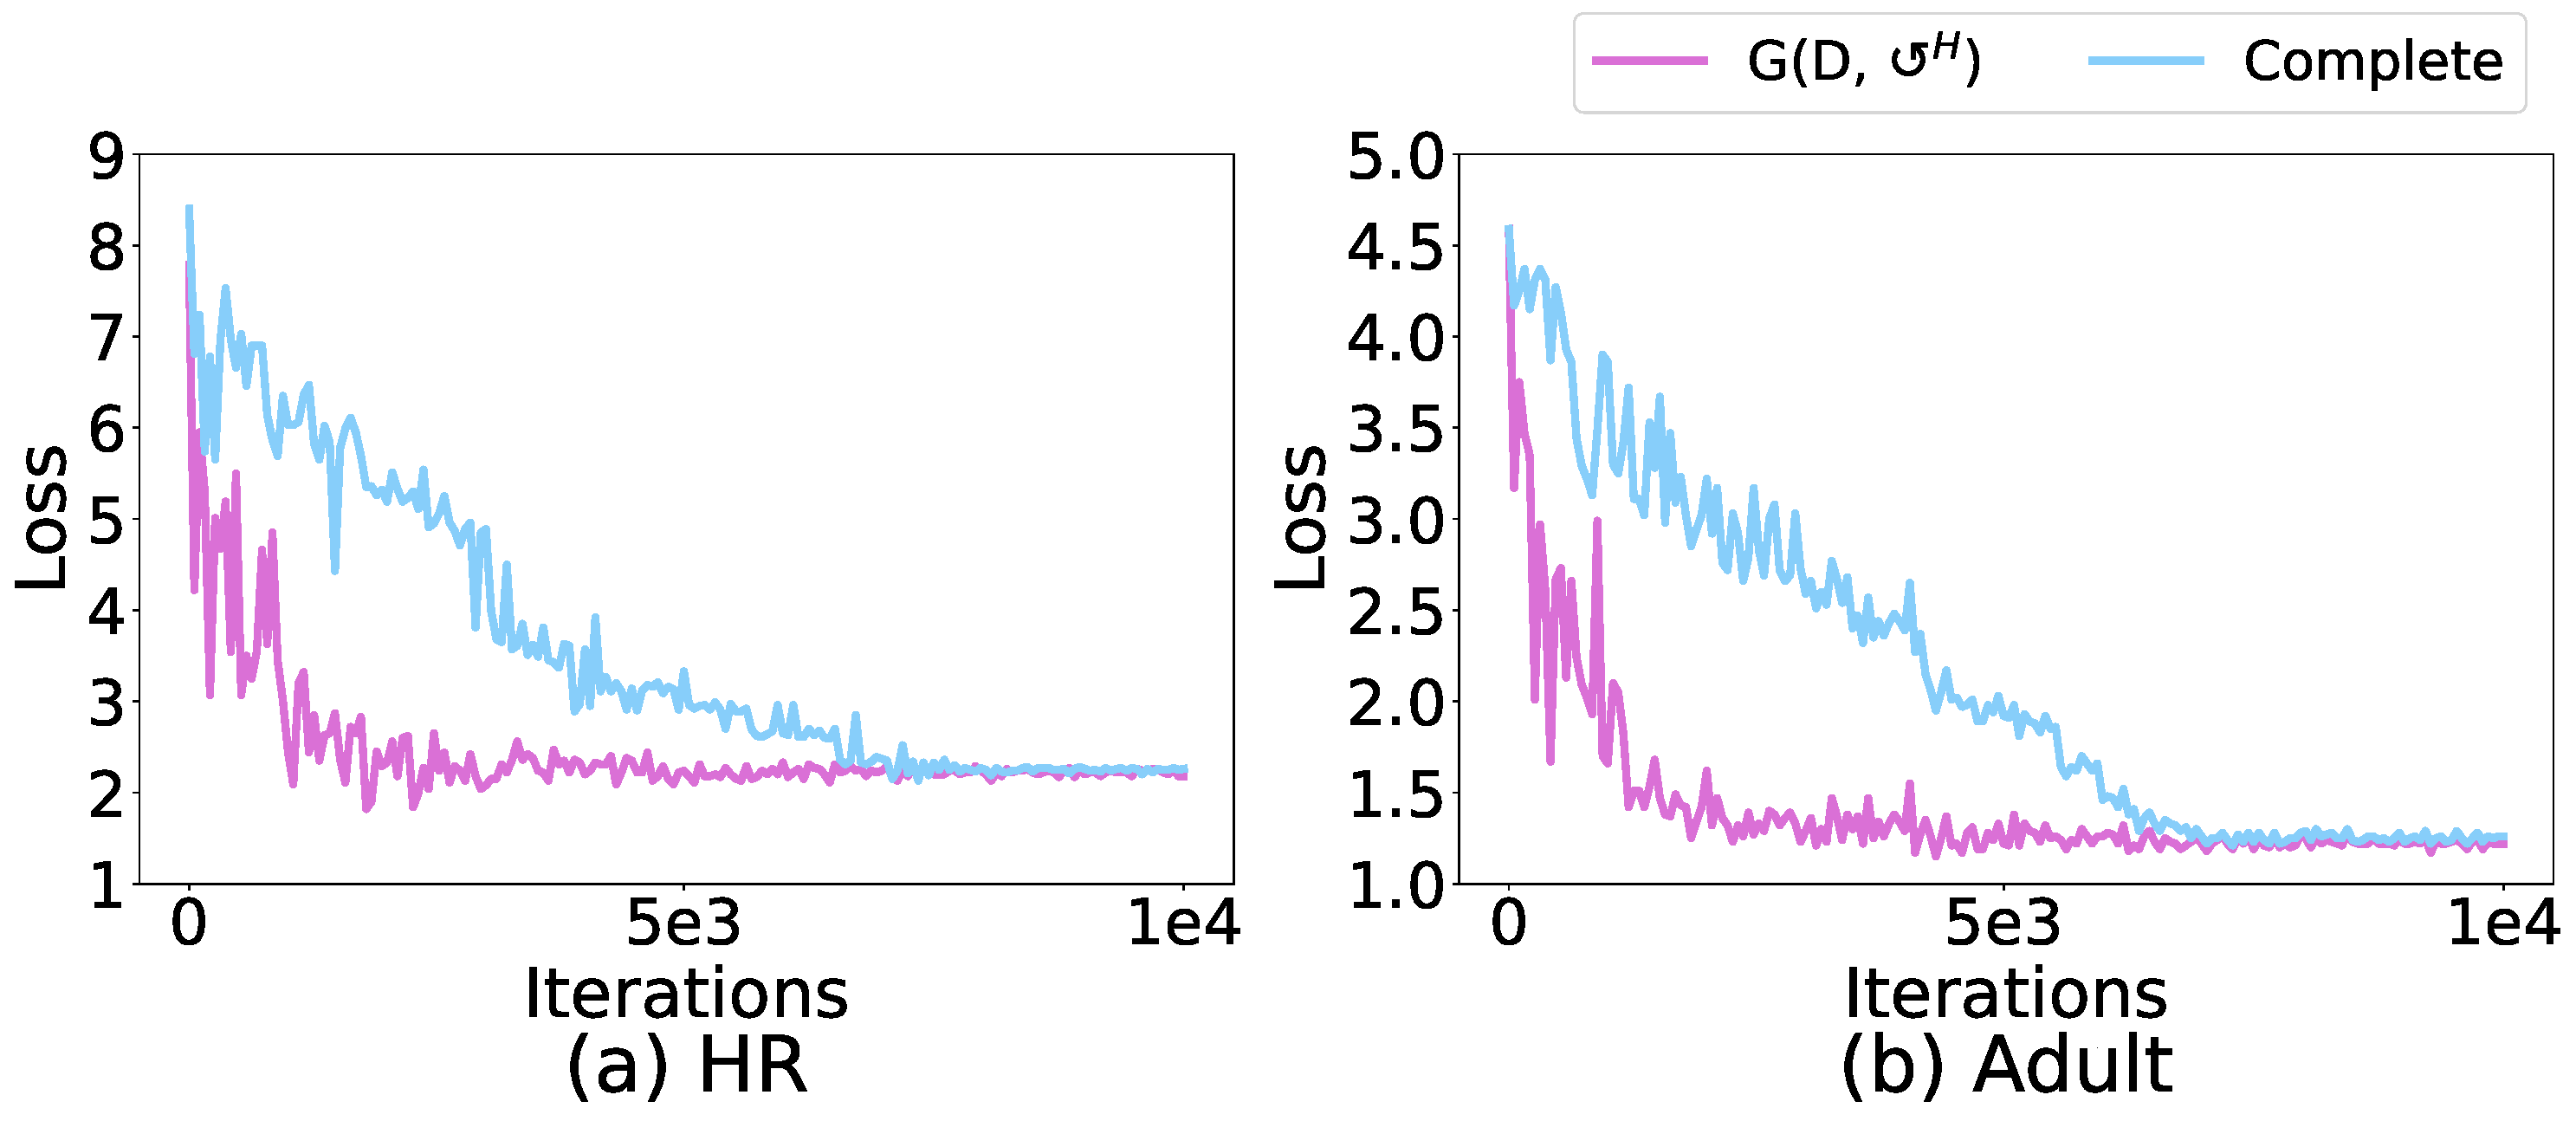
\includegraphics[width=0.5\columnwidth]{figs/realloss}
%	\vspace{-1.5em}
	\caption{Loss of \ours.}
	\label{fig:real_loss}
%	\vspace{-1.5em}
\end{figure}



\begin{figure}[t]   
	\centering
	\begin{minipage}[t]{0.38\textwidth}
		\centering
		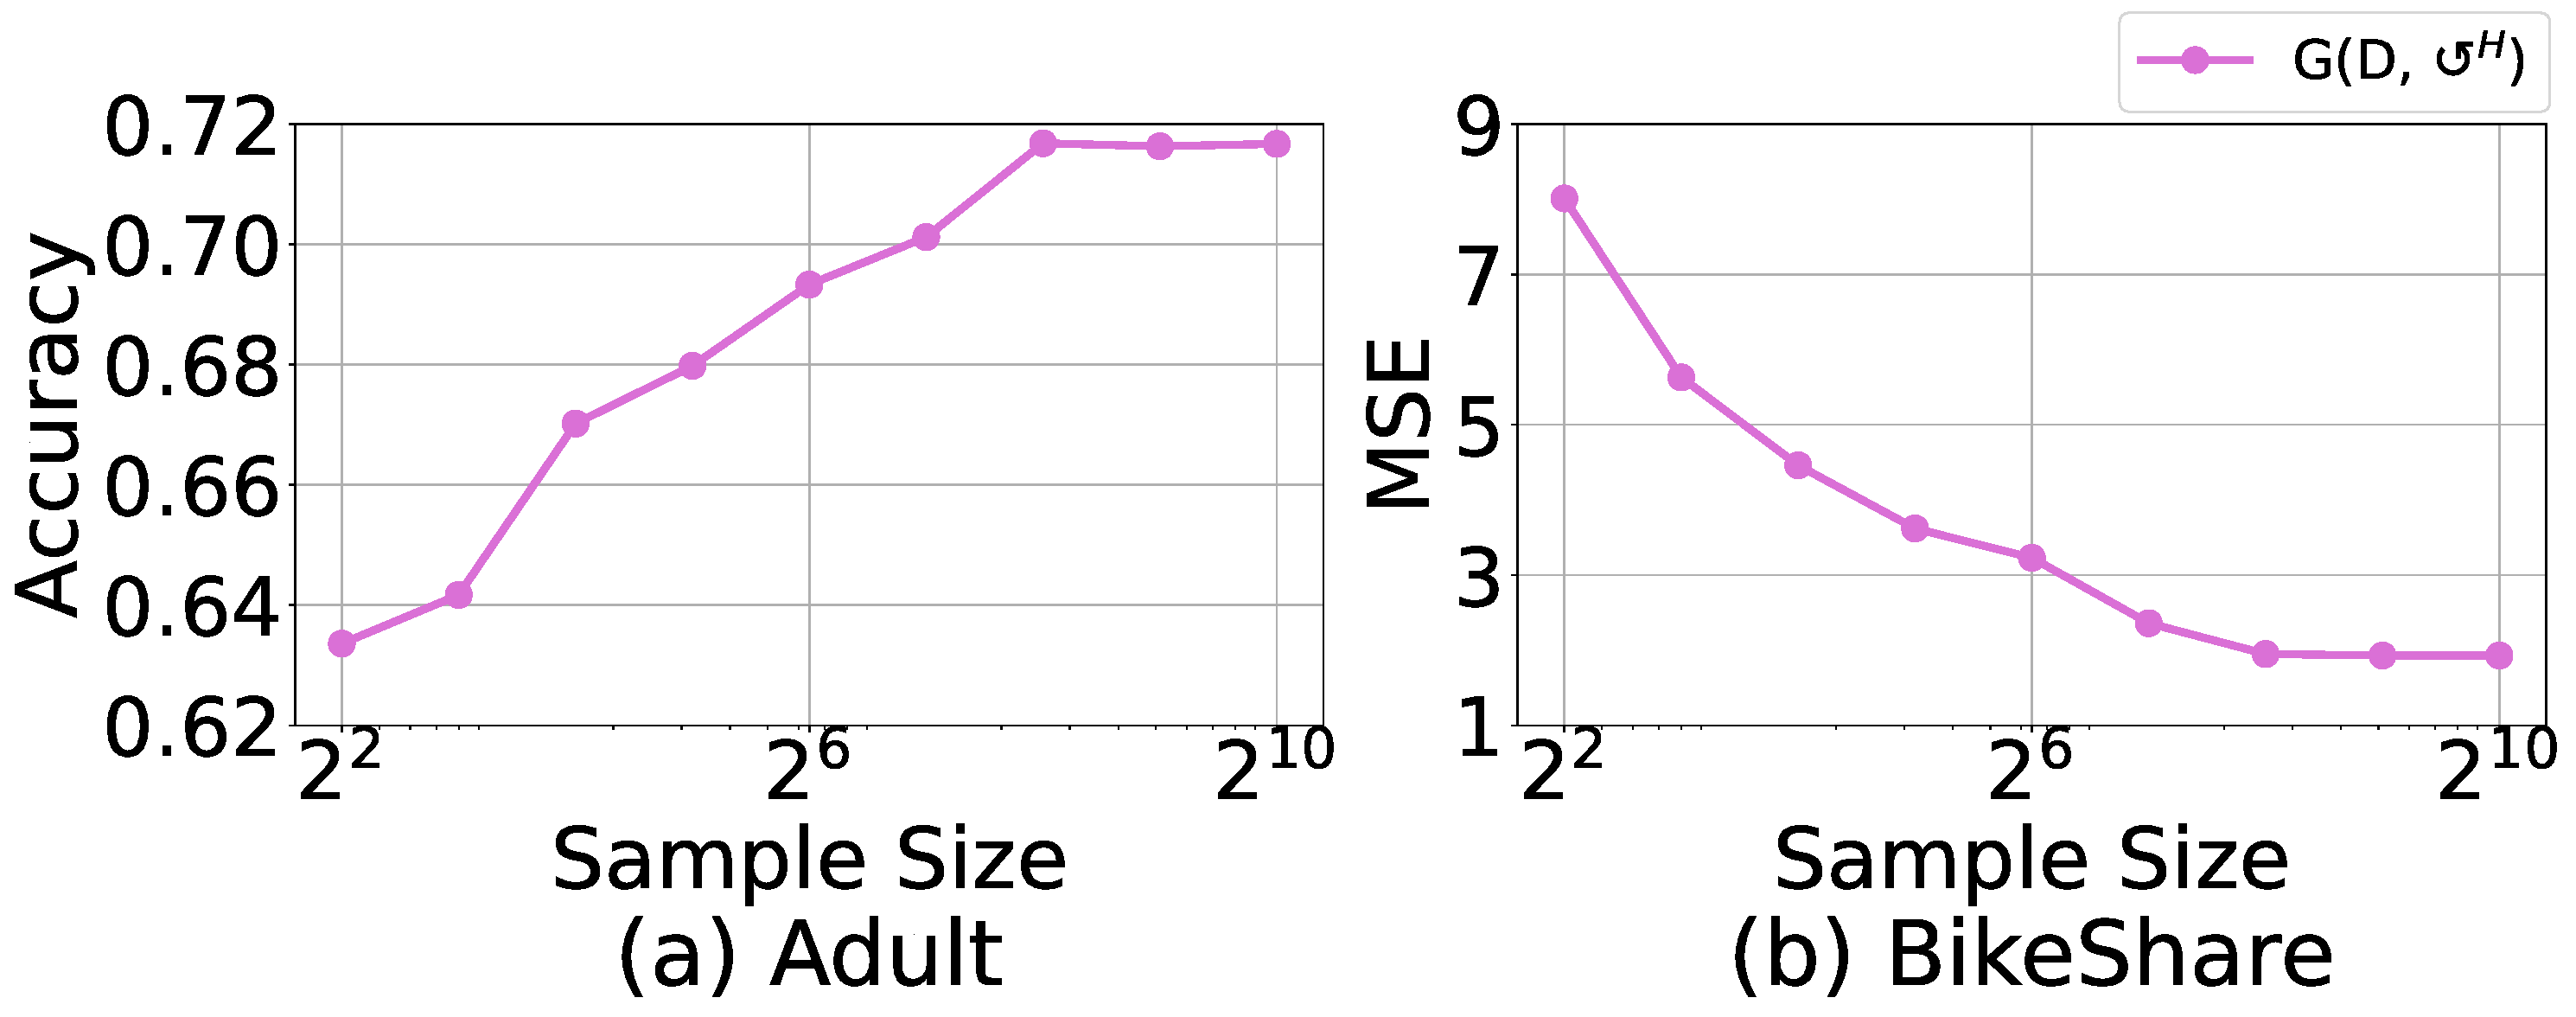
\includegraphics[width=\columnwidth]{figs/samplesize}
		\vspace{-2.5em}
		\caption{Varying sample size.}
		\label{fig:samplesize}
	\end{minipage}
	\begin{minipage}[t]{0.58\textwidth}
		\centering
		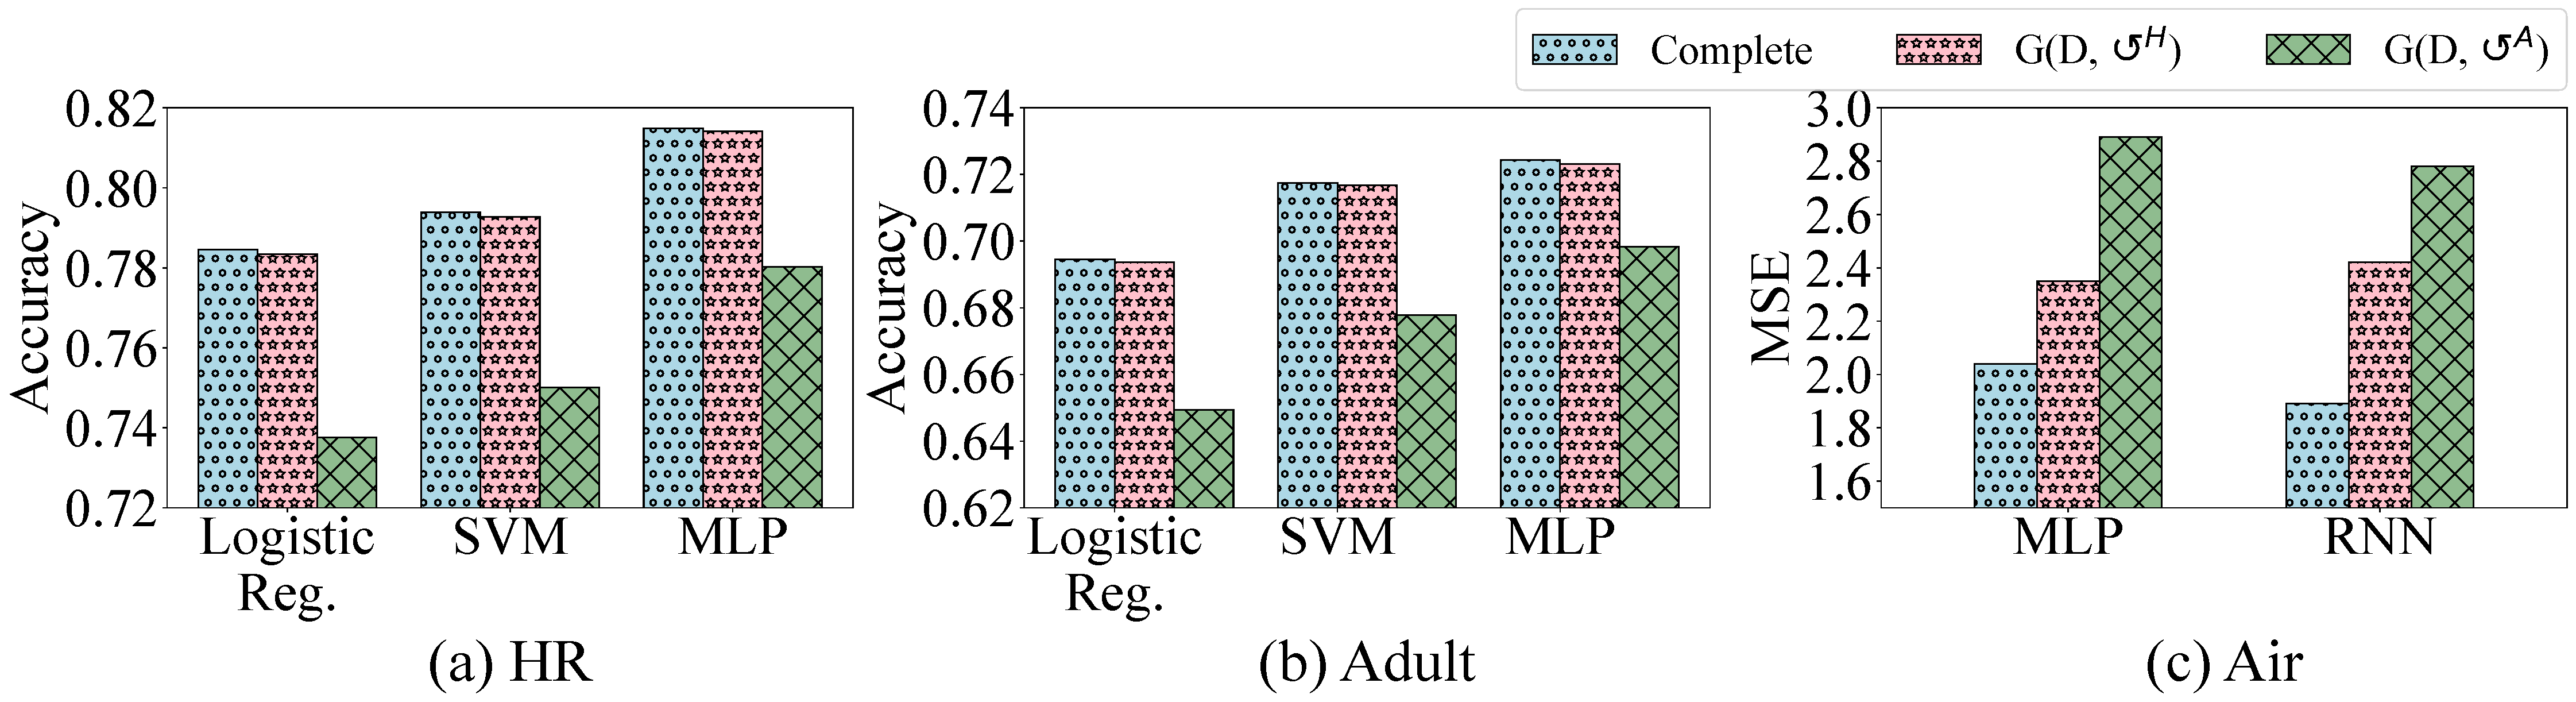
\includegraphics[width=\columnwidth]{figs/downstream_all}
		\vspace{-2.5em}
		\caption{Varying downstream model.}
		\label{fig:downmodel}
	\end{minipage}
	\vspace*{-1.8em}   
\end{figure}



%\begin{figure} 
%	\centering
%	\begin{minipage}[t]{0.48\columnwidth}
%		\centering
%		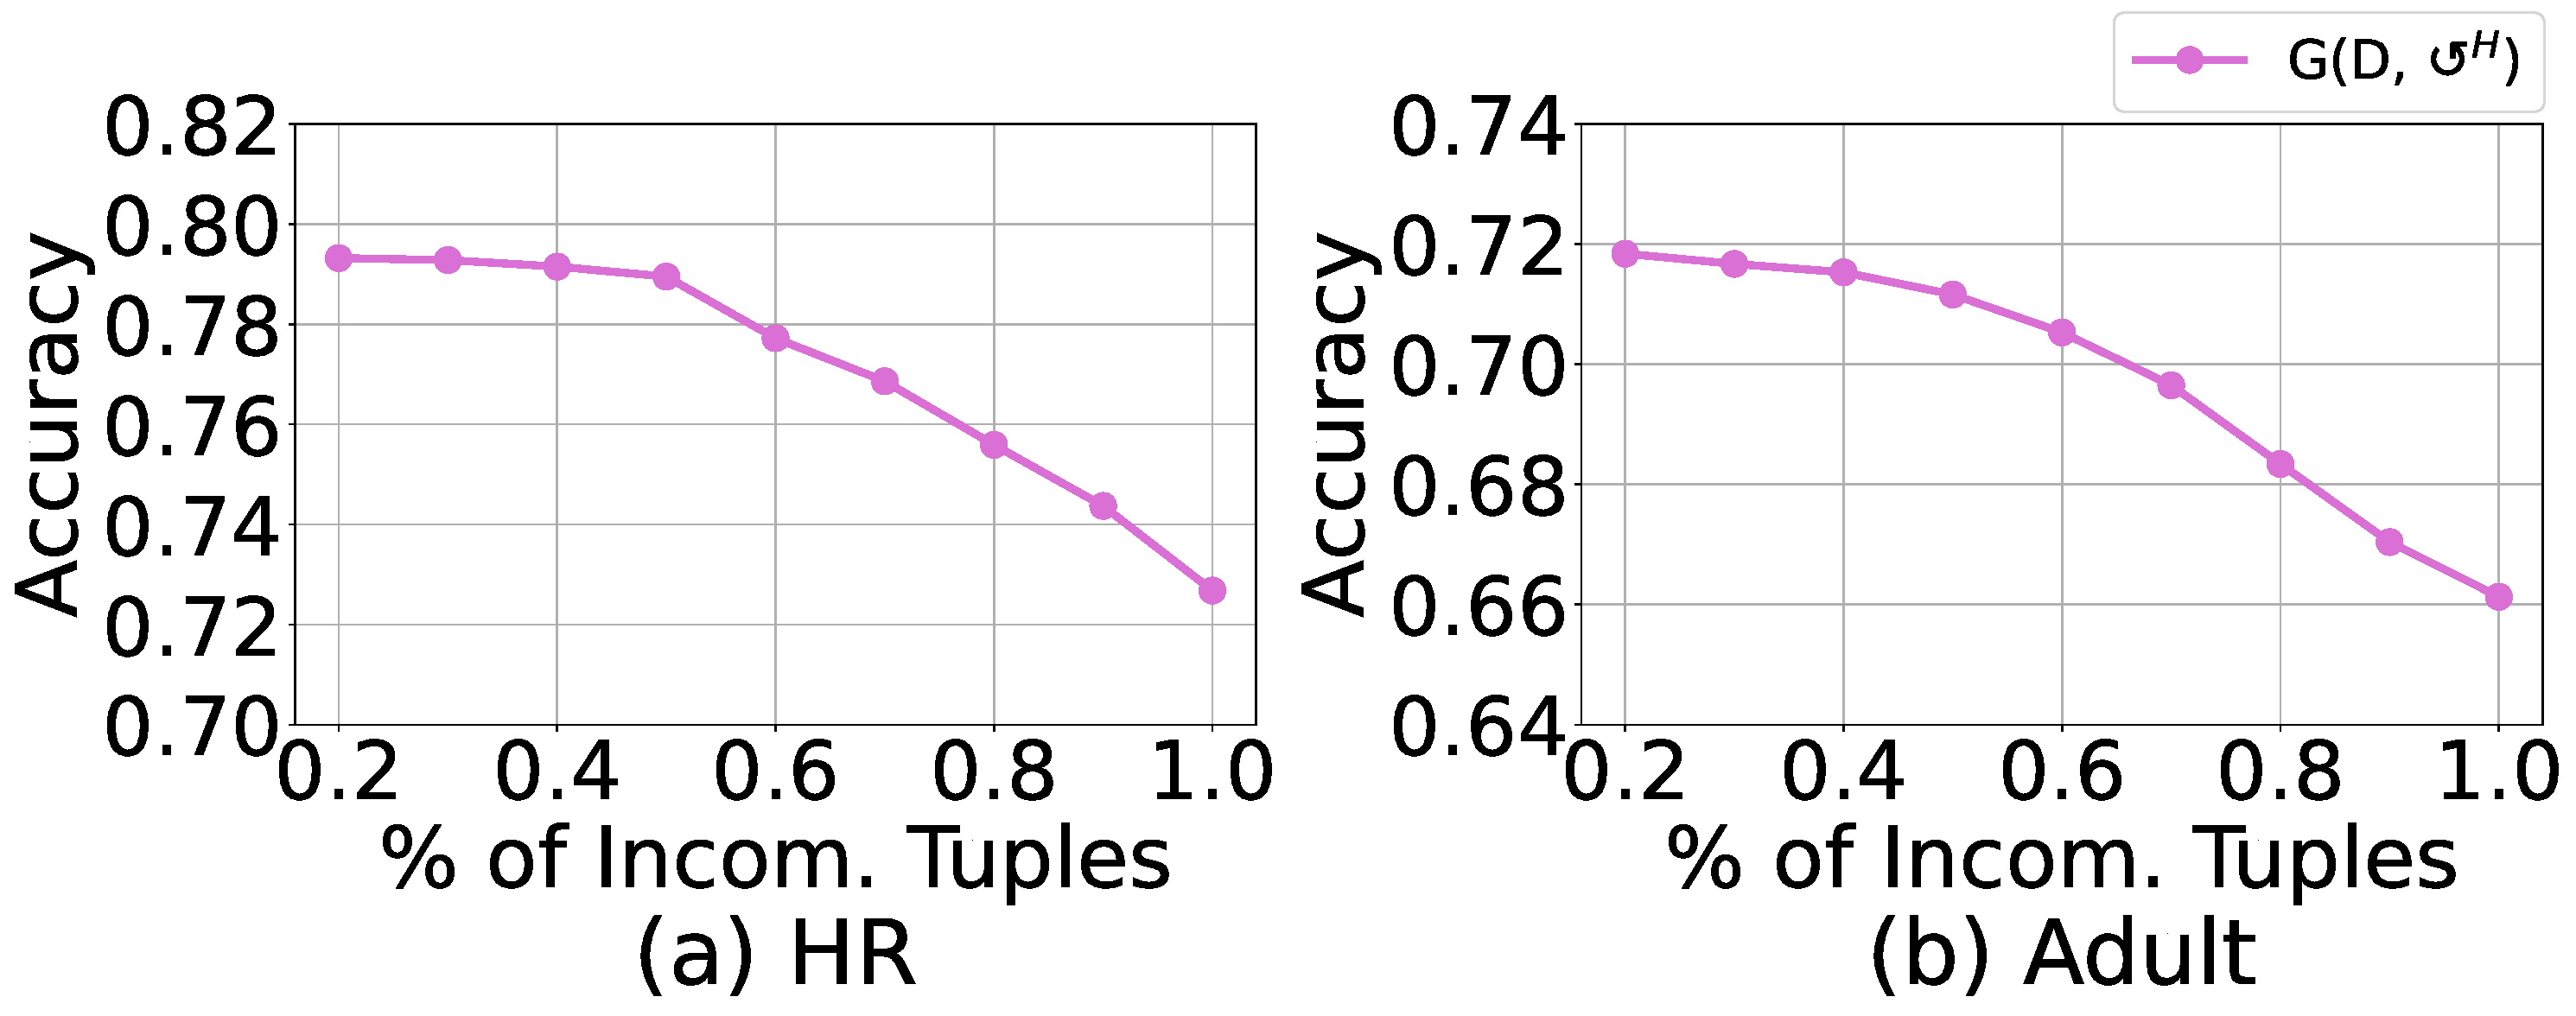
\includegraphics[width=\columnwidth]{figs/missingrate_all}
%		\vspace{-1.5em}
%		\caption{Varying missing tuple rate.}
%		\label{fig:vary_misstuple_all}
%	\end{minipage}
%	\begin{minipage}[t]{0.48\columnwidth}
%		\centering
%		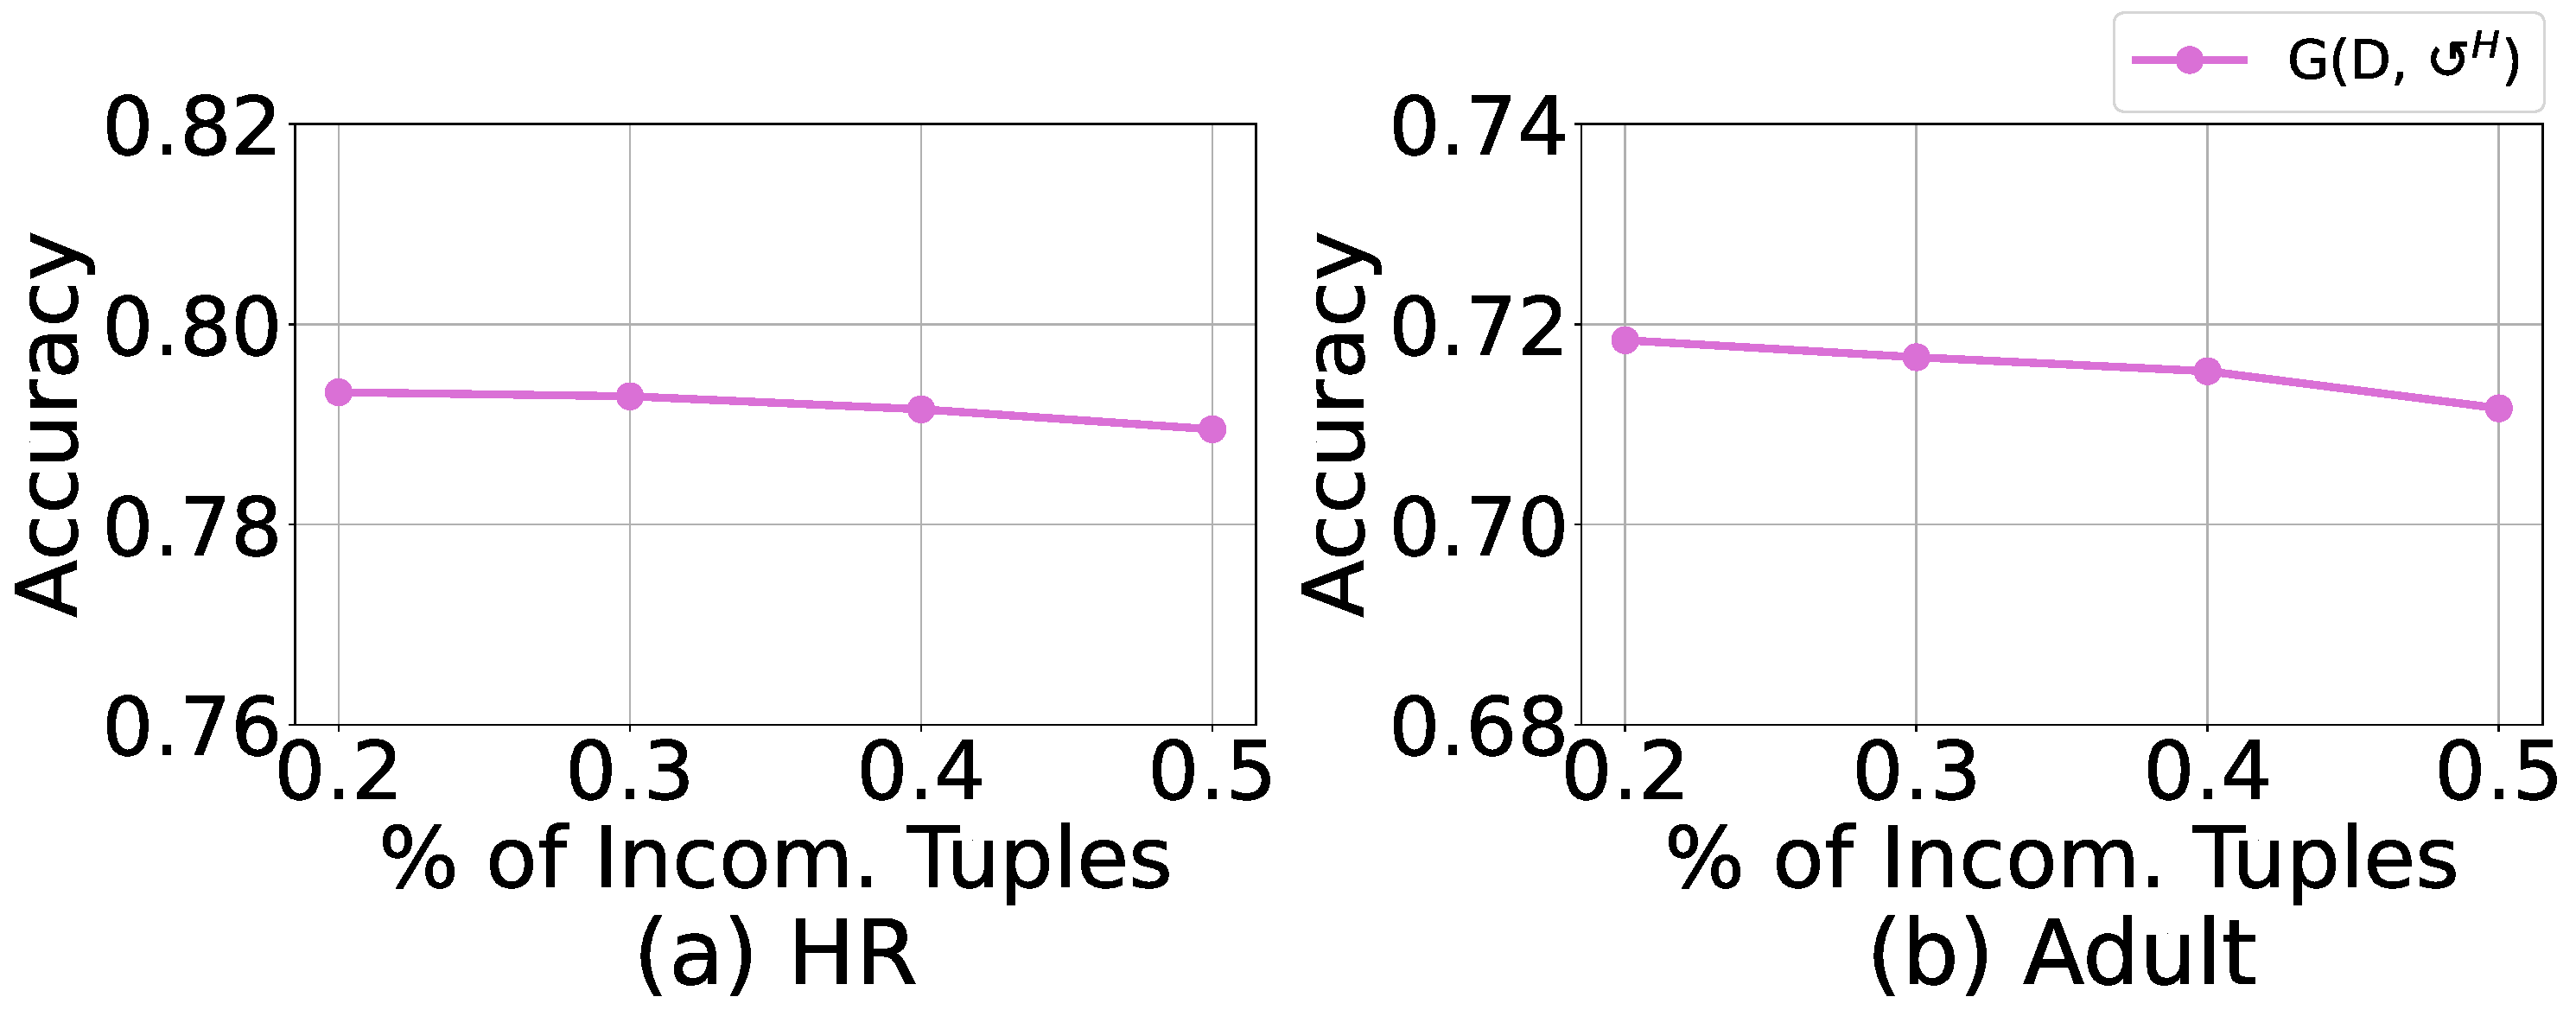
\includegraphics[width=\columnwidth]{figs/missingrate}
%		\vspace{-2.5em}
%		\caption{Varying missing value rate.}
%		\label{fig:missrate}
%	\end{minipage}
%	\vspace*{-1.8em}   
%\end{figure}

\begin{figure}
	\centering
	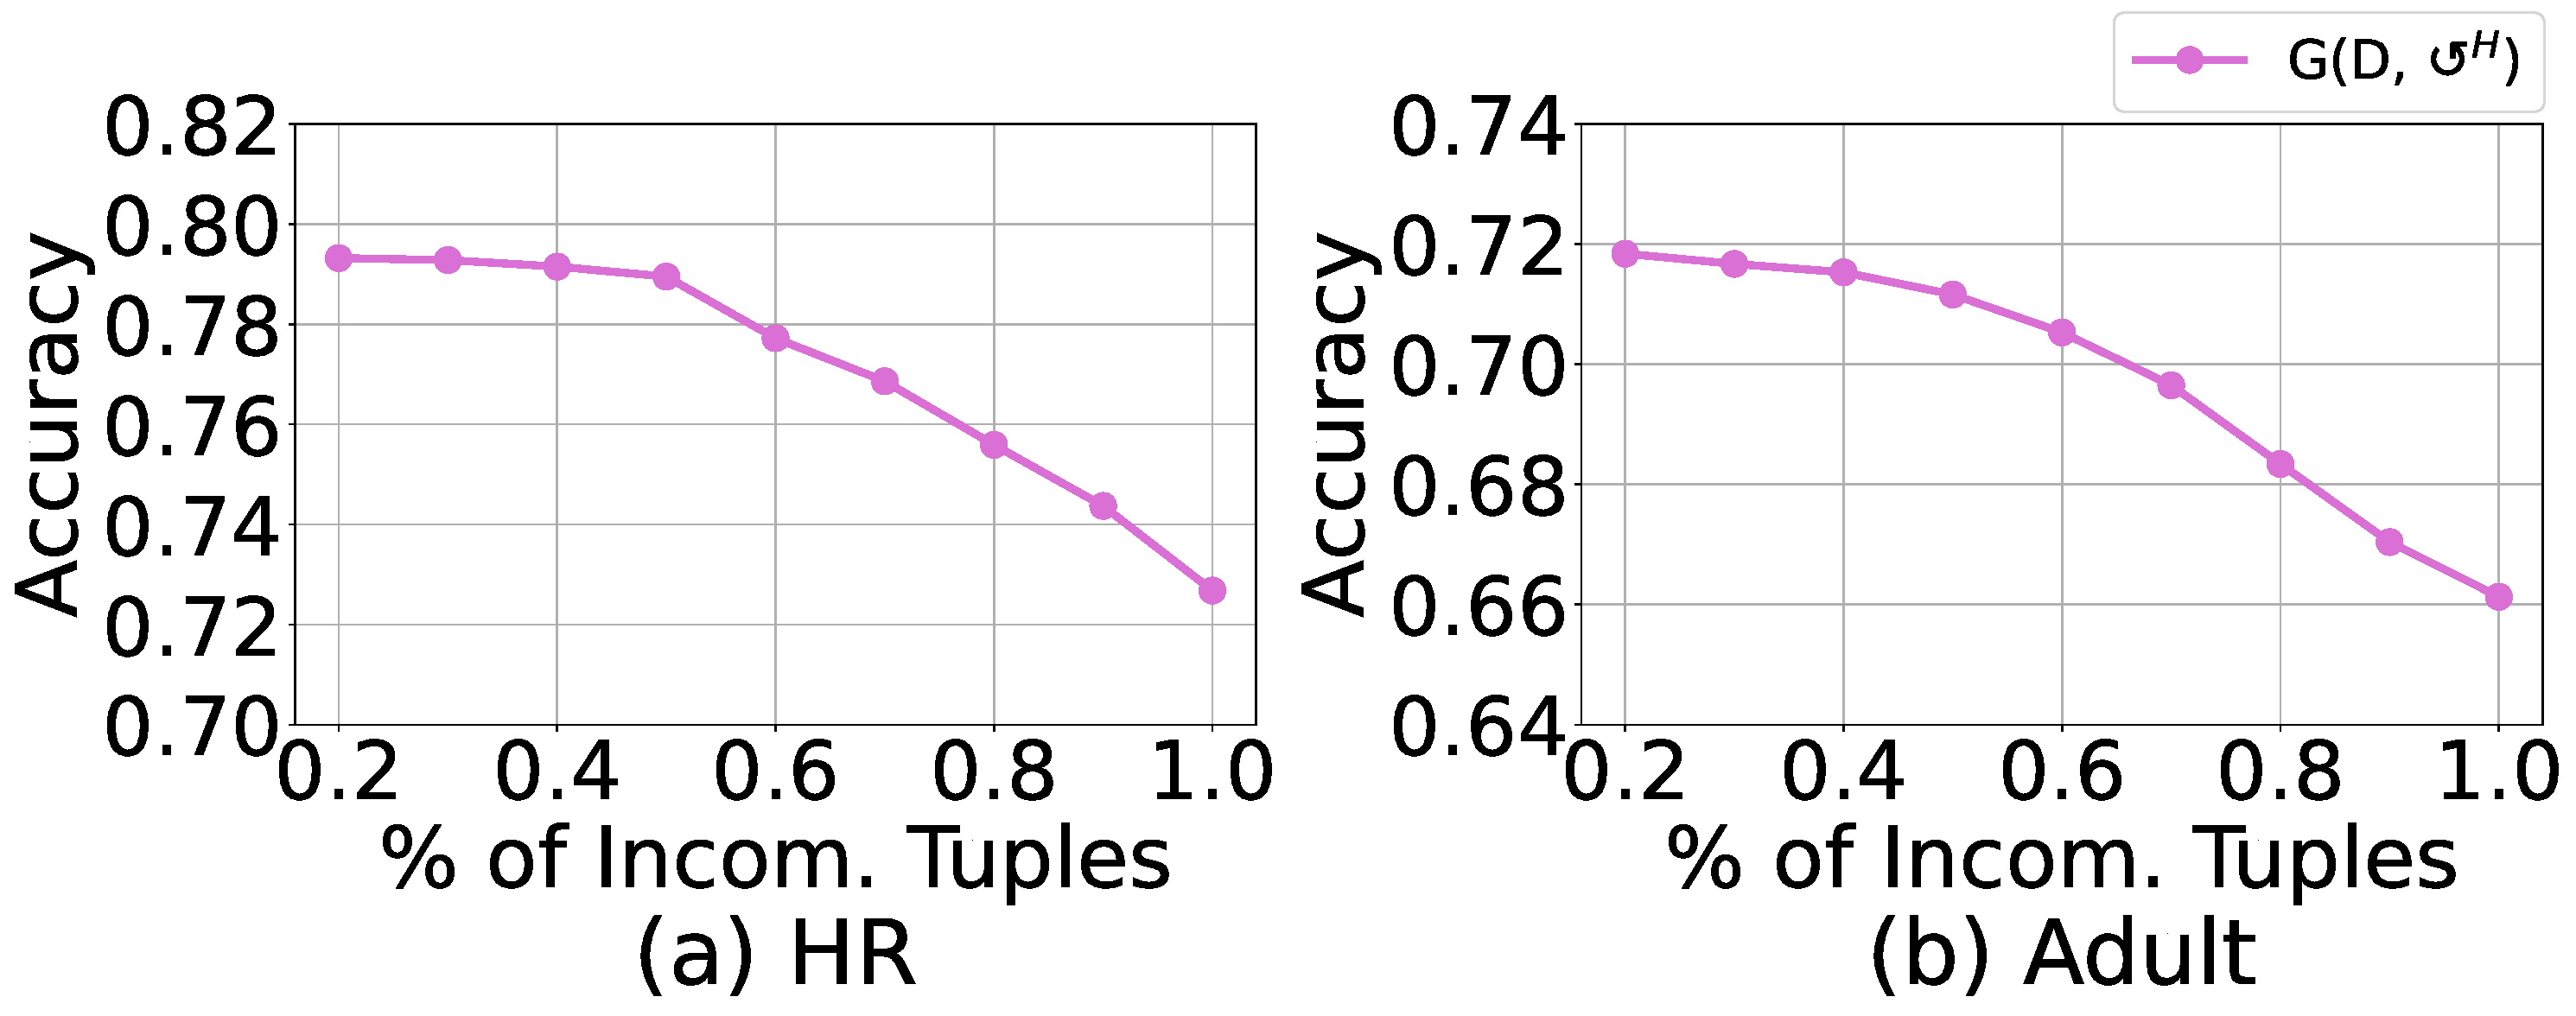
\includegraphics[width=0.5\textwidth]{figs/missingrate_all}
%	\vspace{-1em}
	\caption{Varying missing tuple rate.}
	\label{fig:vary_misstuple_all}
%	\vspace{-1em}
\end{figure}

\begin{figure}
	\centering
	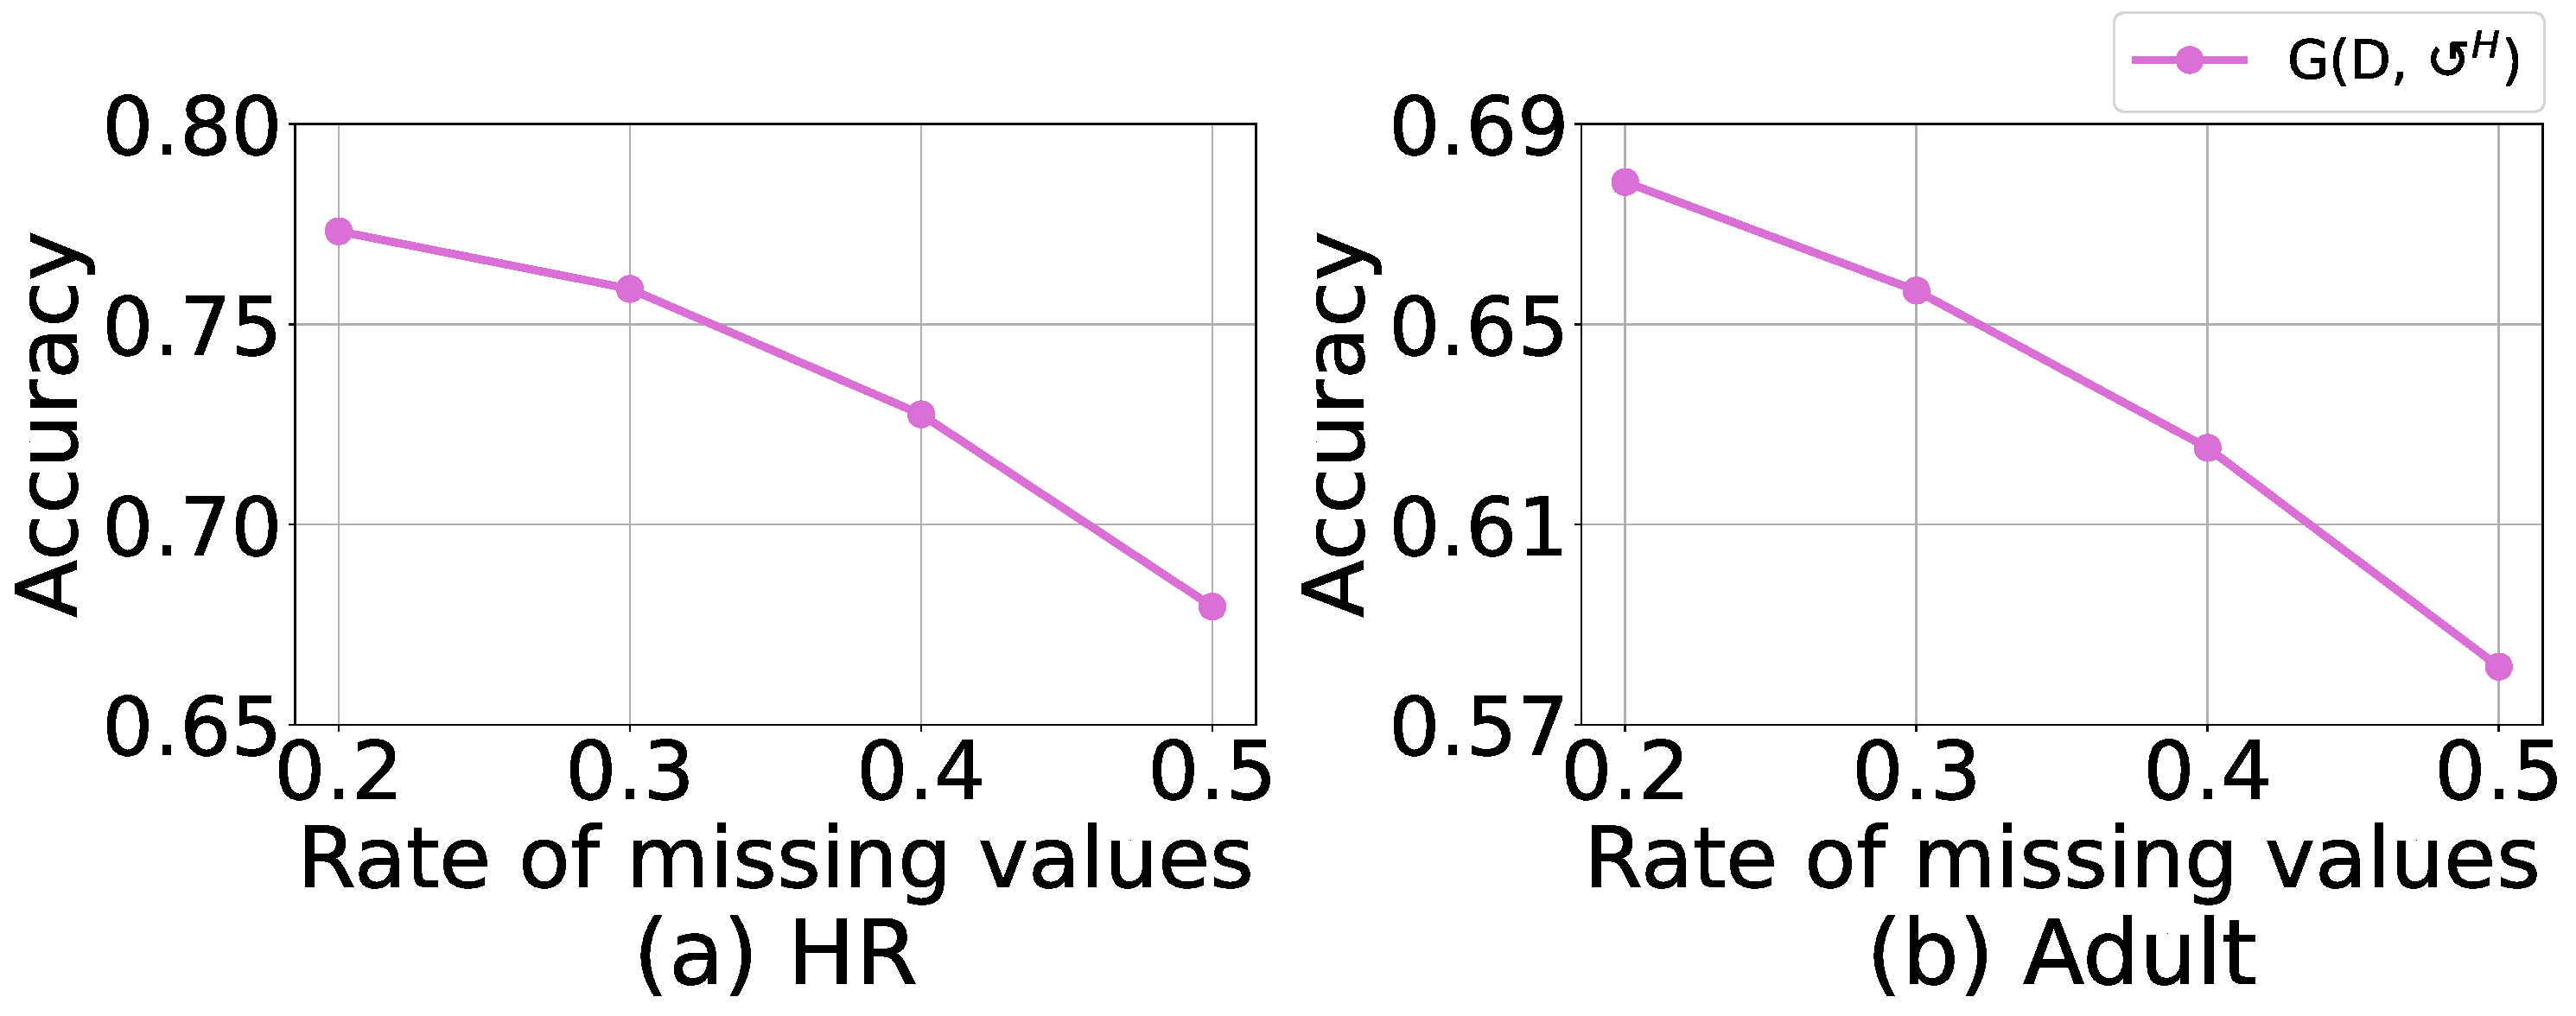
\includegraphics[width=0.5\textwidth]{figs/missingrate_real}
%	\vspace{-1em}
	\caption{Varying missing value rate.}
	\label{fig:realmissrate}
%	\vspace{-1em}
\end{figure}




%\begin{figure*}[t]   
%	\centering
%	\begin{minipage}[t]{0.28\textwidth}
%		\centering
%		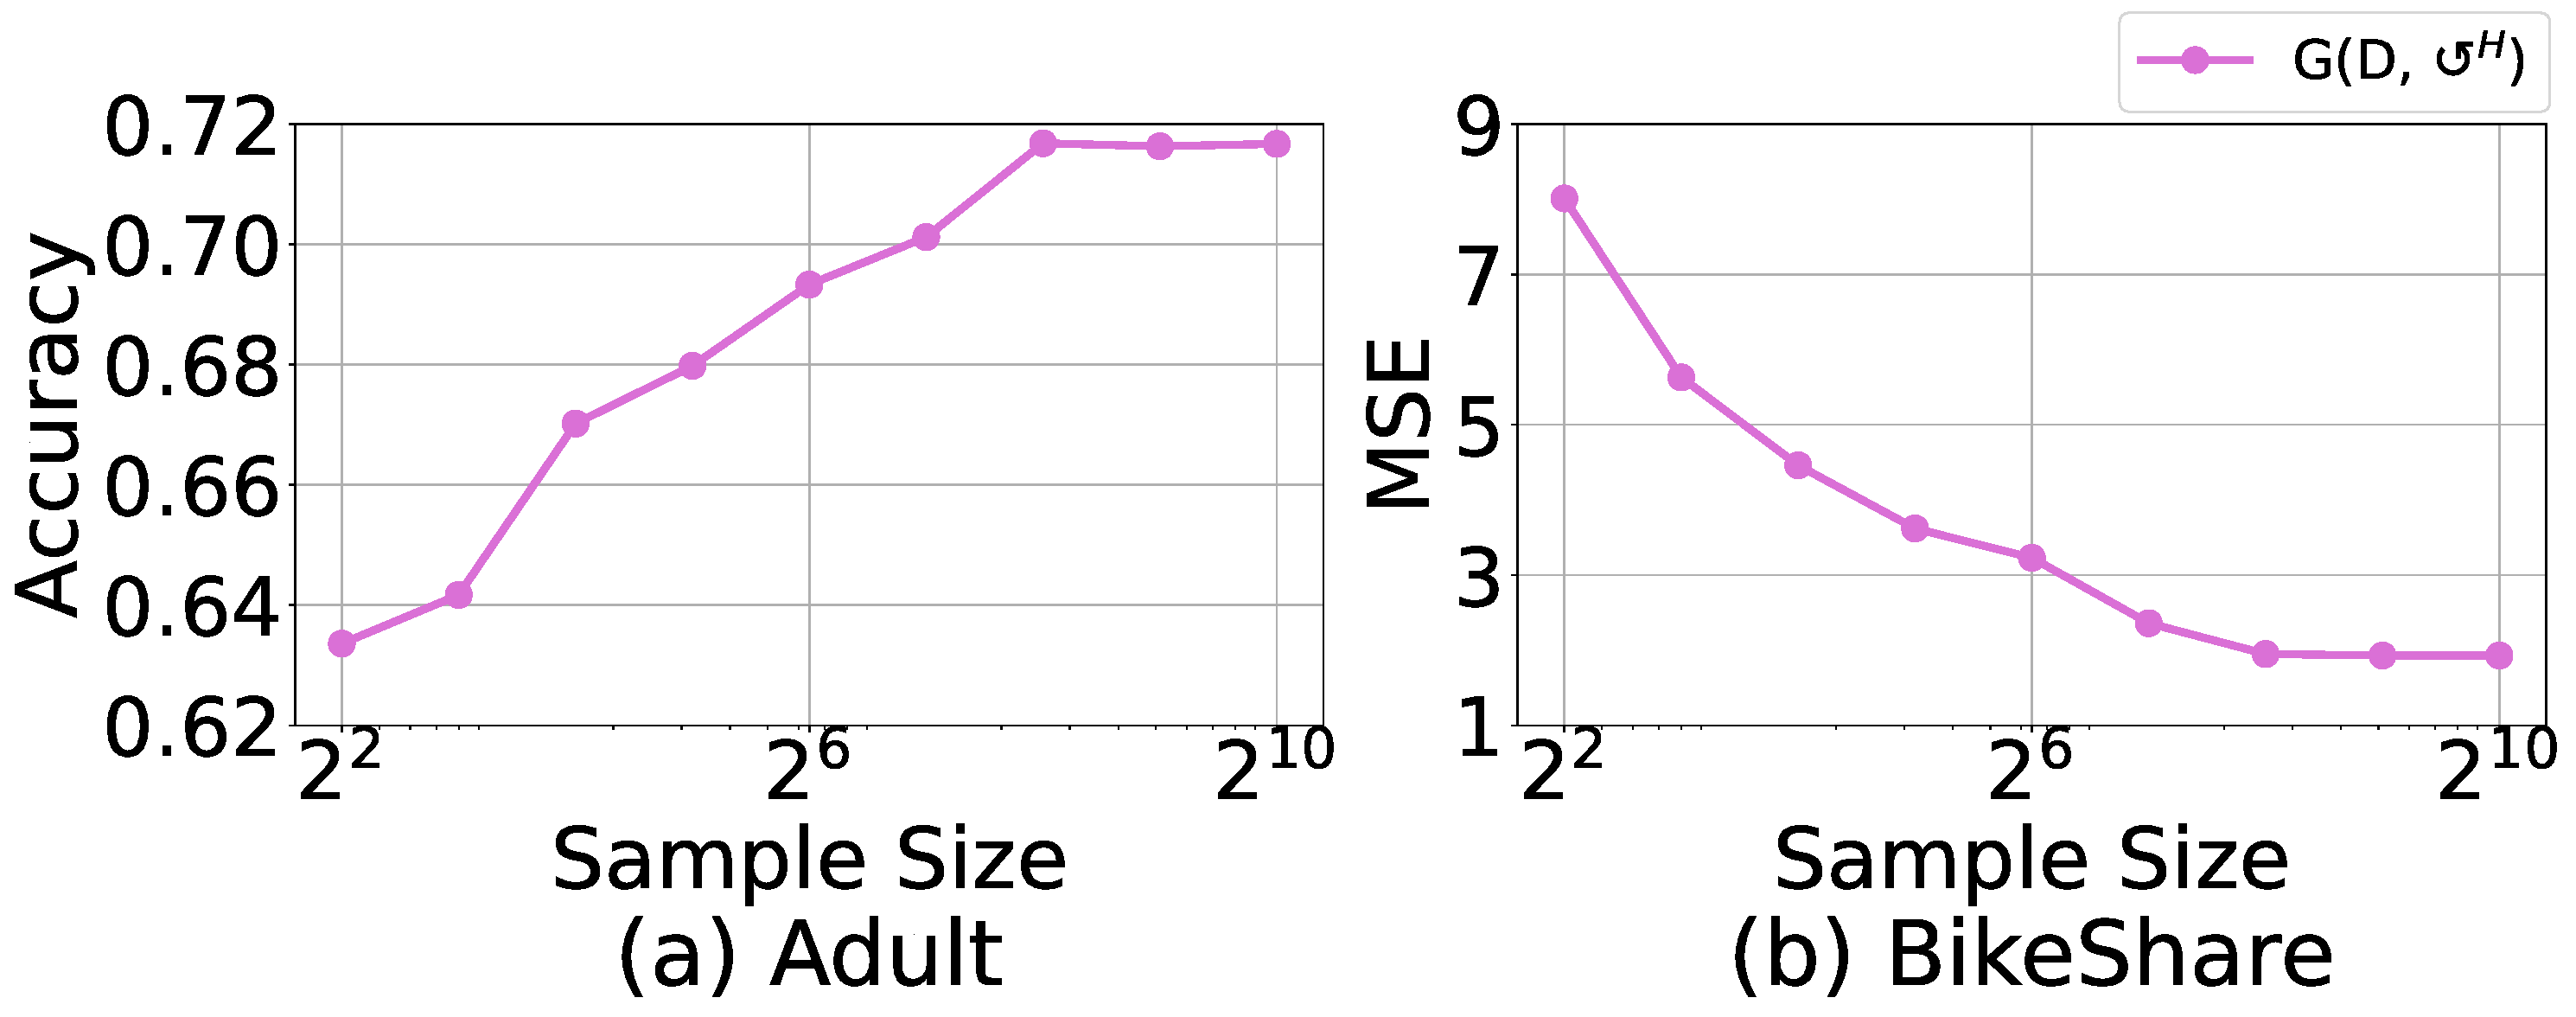
\includegraphics[width=\columnwidth]{figs/samplesize}
%		\vspace{-2.5em}
%		\caption{Varying sample size.}
%		\label{fig:samplesize}
%	\end{minipage}
%	\begin{minipage}[t]{0.43\textwidth}
%		\centering
%		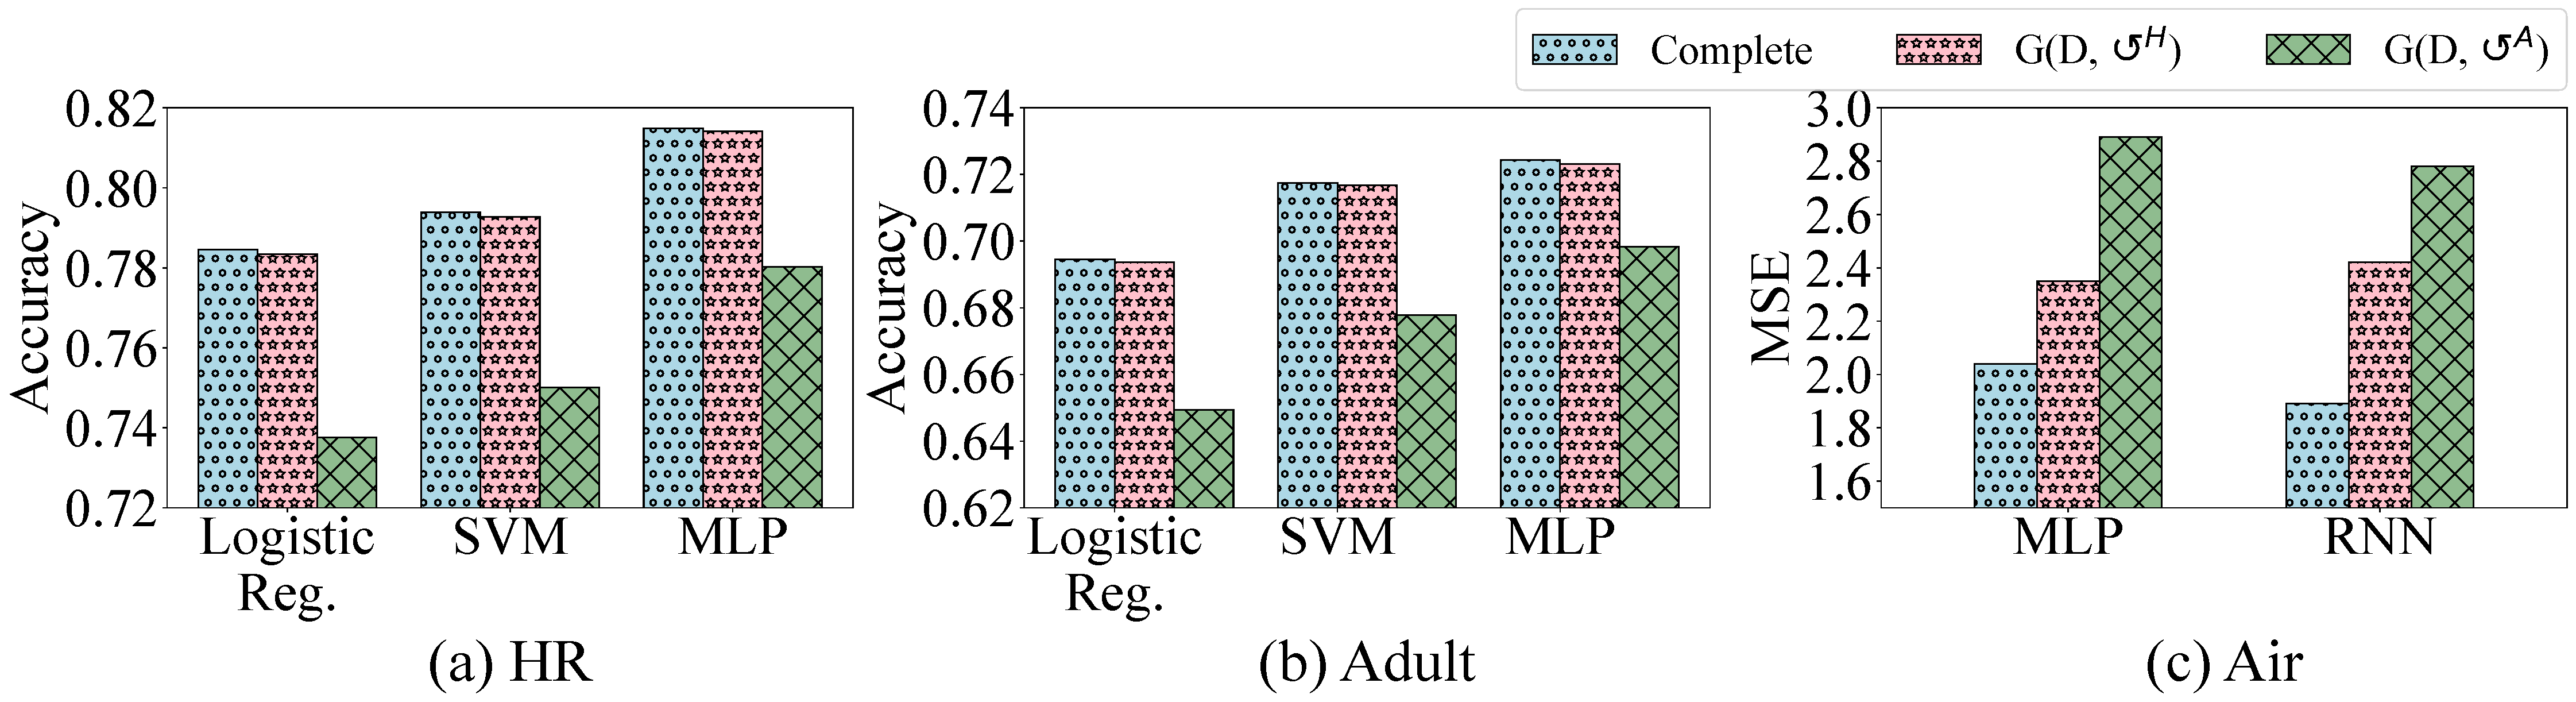
\includegraphics[width=\columnwidth]{figs/downstream_all}
%		\vspace{-2.5em}
%		\caption{Varying downstream model.}
%		\label{fig:downmodel}
%	\end{minipage}
%	\begin{minipage}[t]{0.28\textwidth}
%		\centering
%		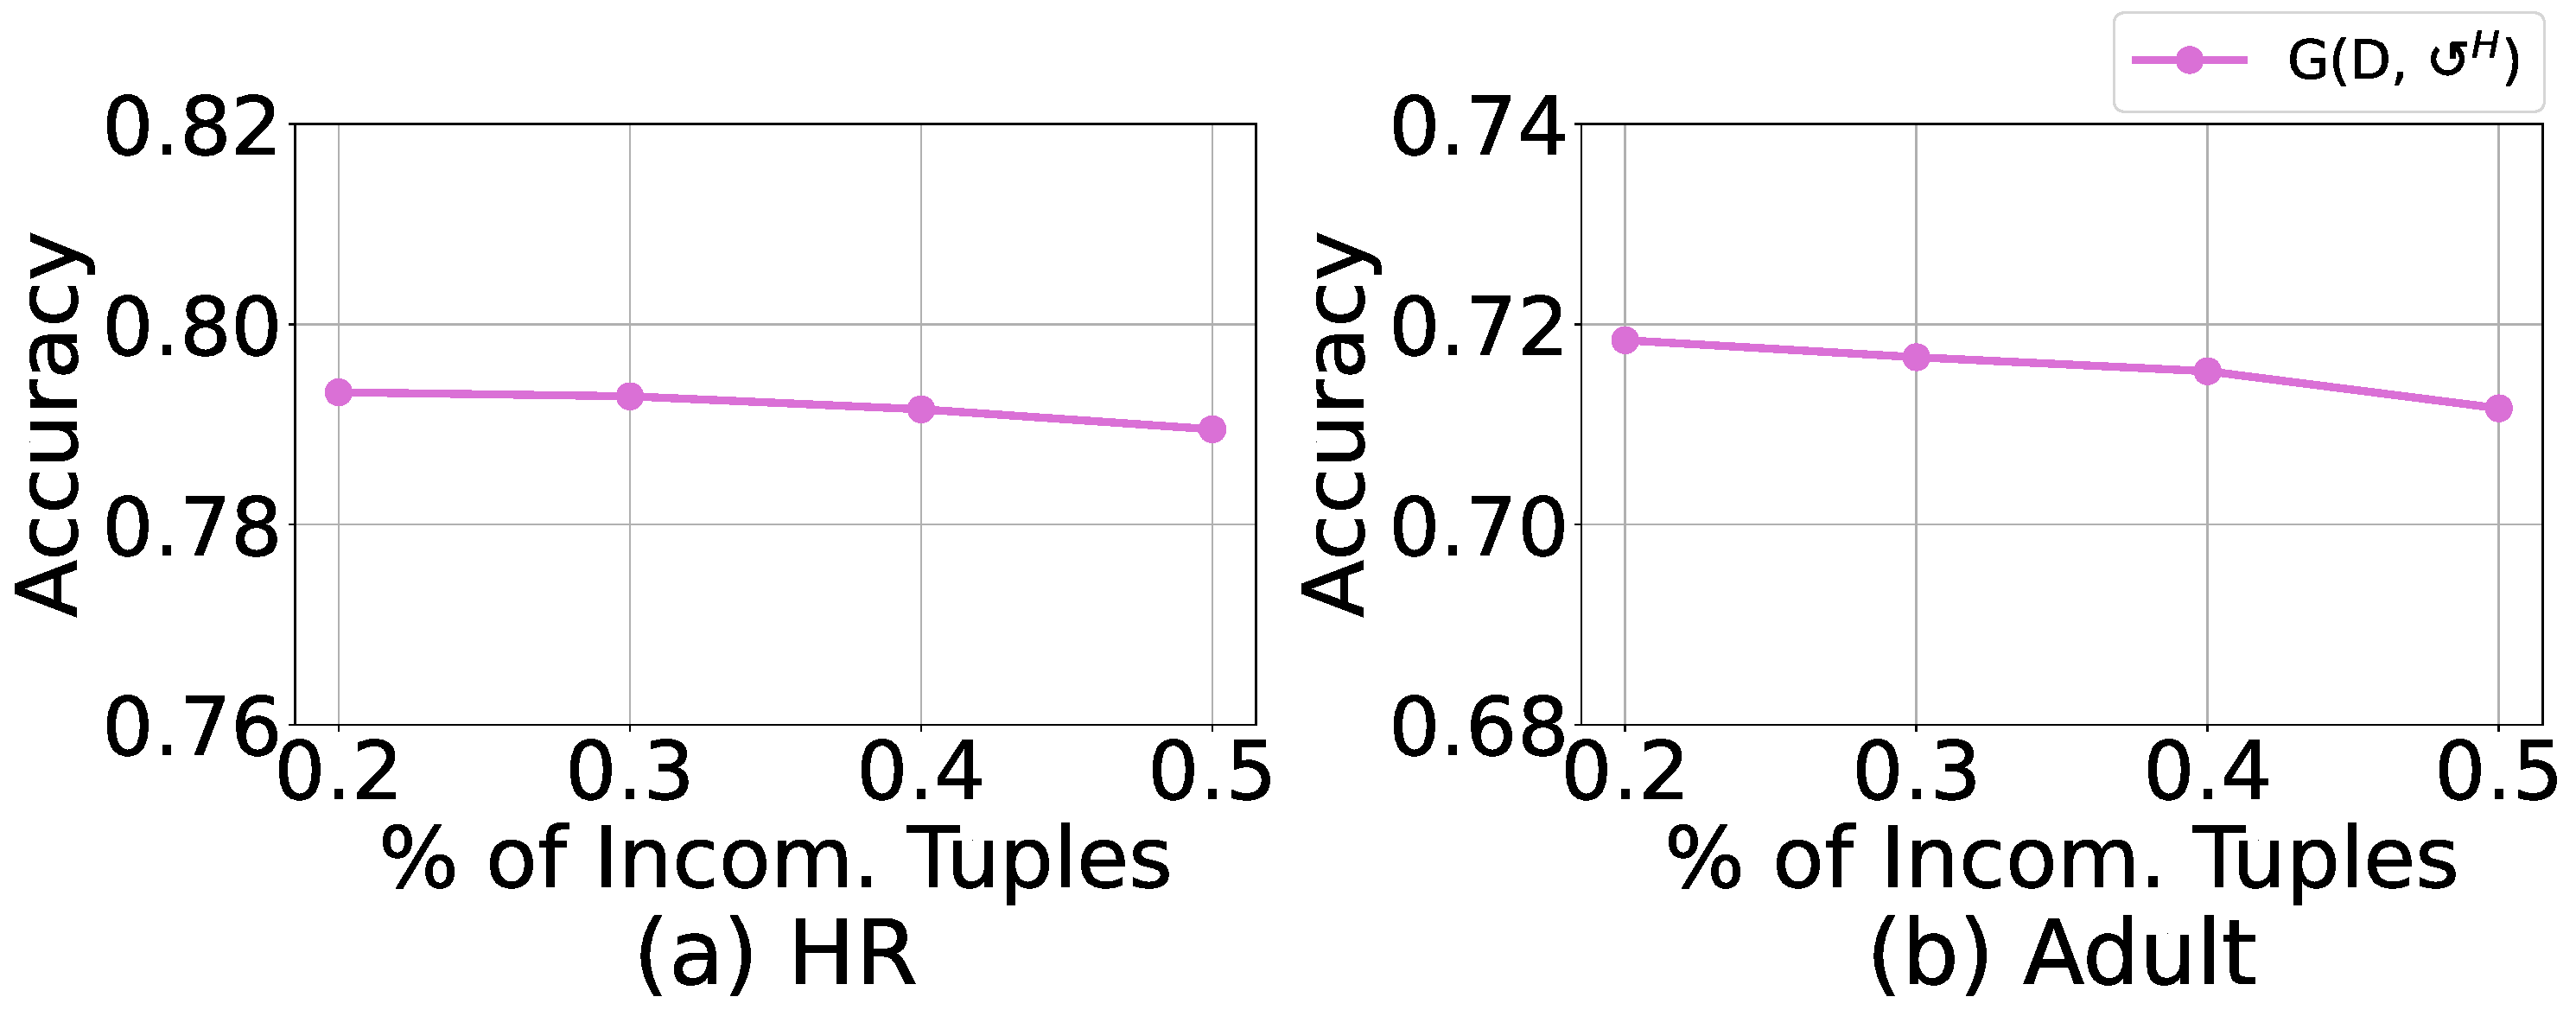
\includegraphics[width=\columnwidth]{figs/missingrate}
%		\vspace{-2.5em}
%		\caption{Varying missing value rate.}
%		\label{fig:missrate}
%	\end{minipage}
%	\vspace*{-1.8em}   
%\end{figure*}

%!TEX root = ../main.tex

\subsection{Batch Algorithm of \ours}
\label{exp:sec:batchalgo}

In Section~\ref{exp:sec:overall}, $\seven$ outperforms other baselines on accuracy, but requires many human iterations. In this part, we evaluate  the batch algorithm of \ours by varying the batch size $b$, \ie Algorithm~\ref{alg:batch} to reduce the number of iterations. Intuitively, the algorithm is  $\seven$  when $b=1$. 
Then we increase $b$ until a single batch with a size $b$ can contain all incomplete tuples in the coreset with size $K$, which is in fact the algorithm $\five$.
 Due to the large number of possible worlds, we adopt the heuristic method in Section~\ref{subsec:batch} to set $l=3$ when $b>1$. 

In Figure~\ref{fig:batchalg}, the $x$-axis denotes the batch size and the $y$-axis denotes the test performance on dataset \adult and  \bike. We can see that when $b$ is small (\ie $b \le 5$), the performance does not significantly decrease (\eg on \adult, the accuracy decrease from 71.7\% to 71.2\%.).  When $b$ keeps increasing, the performance slightly decreases. Thus, \ours is not  sensitive to the batch size $b$ and the Algorithm~\ref{alg:batch} can reduce the number of human iterations without sacrificing much  model performance.


In this part, we also vary the number of possible worlds by varying $l$, which is the number of possibles world per tuple. The larger $l$, the larger number of possible worlds we have. The results are shown in Figures~\ref{fig:vary_l_effect} and  \ref{fig:vary_l_efficient}. In terms of the accuracy, we can see that with $l$ increasing (fixing $b=10$), the accuracy increases first and then  remains stable soon, but the time keeps increasing because more possible worlds indicate more computation. Hence, we do not need a large $l$.

When it comes to the number of possible worlds, we would like to clarify that we do not compare with $\humanfunc(\goodfunc(\train))$ and $\autofunc(\goodfunc(\train))$ because  the number of  possible worlds of $\train$ is very large, which is infeasible to compute. We show the number in Table~\ref{tbl:pwnum}, where we also report the numbers of possible worlds of $\seven$ and $\eight$ in each iteration, which are practical to compute.

 %We use $\sevenbatch$ to denote this method. 

%Instead of asking human to impute one tuple per iteration, we ask the human to impute a small batch of tuples per iteration. We set the batch size $b$ to 3. Besides, we compare $\sevenbatch$ with $\five$ and $\six$. 

%The experimental results are shown in Figure~\ref{fig:batchalg}. We can see that $\sevenbatch$ outperforms other two methods on all datasets. For example, on \adult, $\sevenbatch$ achieves 70.9\% accuracy, while $\five$ and $\six$ achieves 68.4\% and 67.5\%, respectively. This is because $\sevenbatch$ can select more tuples with high utility, that can better represent the train dataset. In addition, $\sevenbatch$ reduced 66\% human iterations comparing with $\seven$ without scarifying too much model performance.

\begin{table}
	\centering
	\caption{The number of possible worlds on different datasets}
	{\small
		\begin{tabular}{cccc}
			\hline
			{\bf Method} & {\bf \nursery} & {\bf \hr} & {\bf \adult} \\
			\hline	
			$\five$ & $10^{201}$ & $10^{201}$ & $10^{202}$ \\
			$\six$ & $10^{201}$ & $10^{201}$ & $10^{202}$ \\
			$\seven$ & $10^3$ & $10^3$ & $10^4$ \\
			$\eight$ & $10^3$ & $10^3$ & $10^4$ \\
			\hline
		\end{tabular}
	}
	\label{tbl:pwnum}
	\vspace{-1em}
\end{table}








%\begin{figure}
%	\centering
%	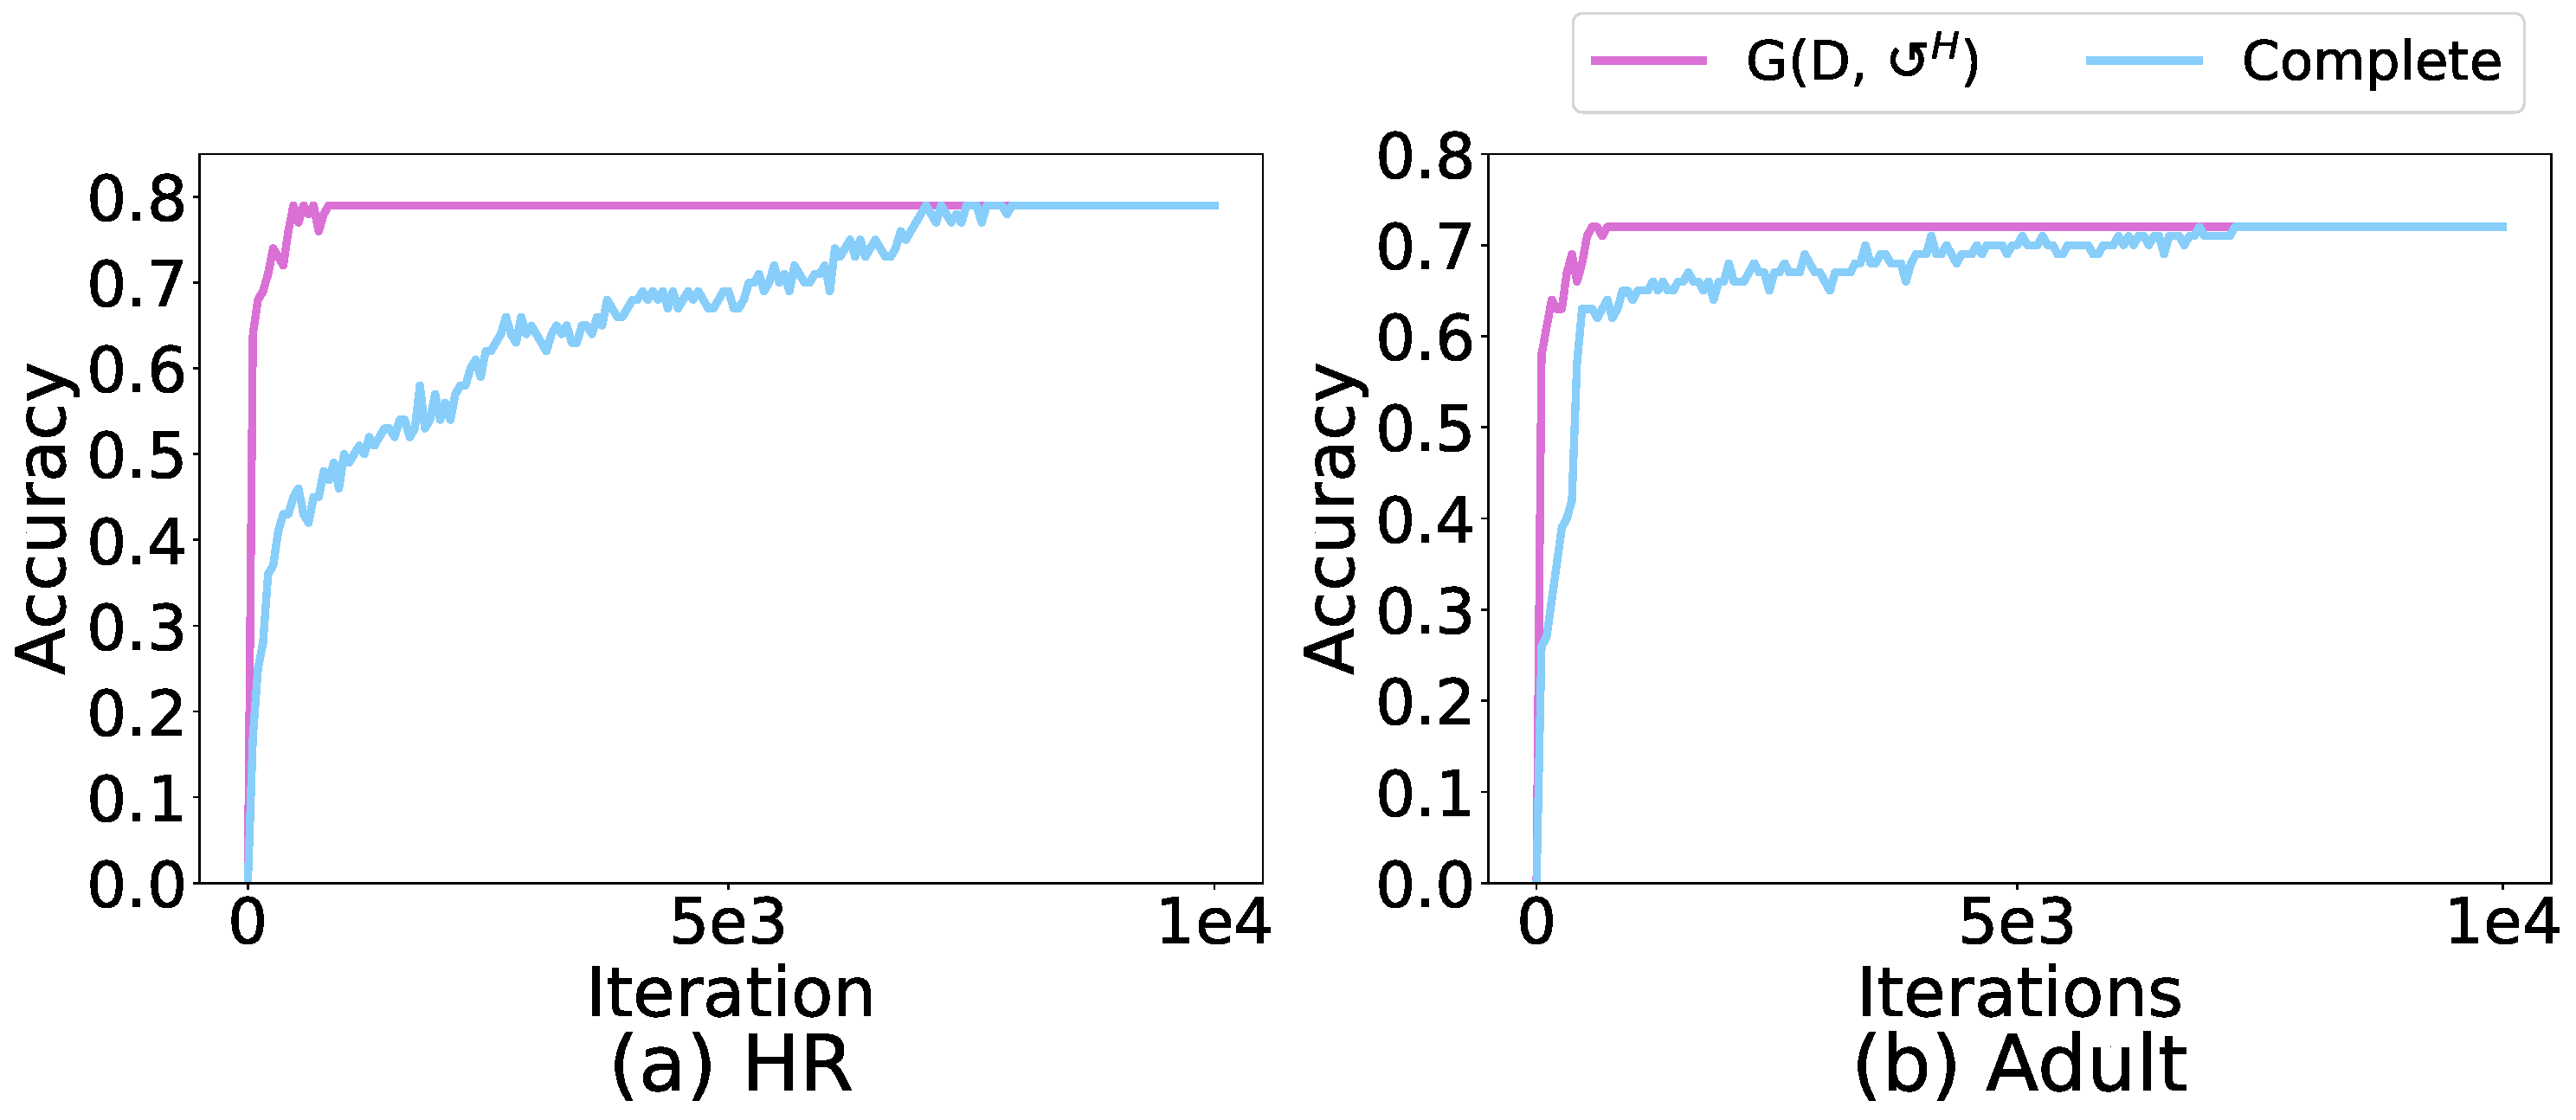
\includegraphics[width=\columnwidth]{figs/converge}
%	\vspace{-2em}
%	\caption{Convergence of \ours.}
%	\label{fig:converge}
%\end{figure}


%!TEX root = ../main.tex
\vspace{-0.5em}
\subsection{Convergence Evaluation}

In Section~\ref{sec:proof}, we have shown  the convergence rate of \ours theoretically. In this part, we test the convergence of training over the coreset ($\seven$) and entire data (\truth) empirically.  Figure~\ref{fig:converge} shows the test accuracy of two methods with the number of training iterations increasing. We can observe that on both datasets, training on the coreset converges much faster than training on the full data. 
For example, on dataset \adult, it takes $\sim$40 iterations for \ours to converge, which is  $180\times$ faster than {\truth}. This is because \ours has the same convergence rate with training over the entire dataset as discussed in the theoretical result of Section~\ref{sec:proof}, but the entire dataset (\eg  ~\adult) is $200\times$ (similar to $180\times$) larger than the coreset ($\rho=0.005$).
 That is, \ours converges with the same number of epochs  as training on the entire dataset. Since the size of coreset is much smaller, \ours is more efficient. Also, we can achieve competitive accuracy as training on full data by approximating the full gradient with a theoretical bound. 
 

%\add{Figure~\ref{fig:real_loss} also shows the cross entropy loss of two methods with the number of iterations increasing. We can obtain the actual convergence rate from Figure~\ref{fig:real_loss} and compare it with the theoretical value. For example, at the $1^{st}$, $5^{th}$, $10^{th}$ epoch, we find that the actual convergence rates are 6.77, 3.25 and 1.26. The theoretical convergence rates are 8.4, 3.8 and 2.7.}

Furthermore, we report the loss change to reflect the relation between  actual convergence rate and theoretical results. In Figure~\ref{fig:real_loss}, on dataset \adult, the initial loss is 8.4. According to the theoretical convergence rate $O(\frac{1}{\sqrt{k}})$ (this $k$ denotes the $k$-th epoch),  the loss should decrease to around 3.8 at the end of 5-th epoch ($\approx$ 3200-th iteration). Actually,  the  actual loss decreases to 3.25 at that time, which is close to the theoretical value.

 %Thus, \ours needs the same number of epochs to converge as training on the entire dataset. Since the size of coreset generated by \ours is much smaller than the entire dataset, training on the coreset needs much smaller number of iterations to converge.  \cc{proves what? the result shows what? }In this part, we evaluate the convergence of \ours.  Figure~\ref{fig:converge} shows the performance on test dataset for $\seven$ and {\truth} with increasing SGD iterations. \cc{what does the iteration mean? epoch??} {\truth} reflects the convergence on the whole train dataset. We can see that training on the coreset select by \ours is much faster than on the whole train dataset. On dataset \adult, it take about 60 iterations for \ours to converge, which is nearly $120\times$ faster than {\truth}. Besides, the performance of our method is competitive to {\truth}. That is to say, we can make the training process more efficient and without scarifying model performance. 
%!TEX root = ../main.tex
\vspace{-0.5em}
\subsection{Sensitivity Analysis}
\label{exp:sec:sensitivity}

\noindent{\bf Varying the sample size.} In this part, we vary the sample size $h$ and evaluate the performance. The experimental results are shown in Figure~\ref{fig:samplesize}. We vary the sample size $h$ from $2^2$ to $2^{10}$. We can see that when $h$ is too small, the performance is low. The reason is that \ours cannot precisely estimate the utilities of tuples when $h$ is  small.  When the sample size increases, we can see that the performance improves rapidly and finally becomes stable, which indicates that \ours is not much sensitive to the sample size when $h$ is not too small.



\noindent{\bf Varying the downstream models.} Recap that \ours can be used on different convex models. Thus, in this part, we apply \ours on different convex models and evaluate the performance. We evaluate logistic regression and SVM for classification tasks. For regression tasks, we evaluate linear regression, ridge regression and SVM regression. We can see that  in Figure~\ref{fig:downmodel} (a) and (b), on dataset \adult, $\seven$ achieved 71.7\% accuracy for SVM, better than on logistic regression (69.4\%). Although different downstream models may have different performance, \ours can improve the model performance for the specific downstream model. In order to show that \ours can be used for other types of models like neural networks, we compare with Multilayer Perceptron (MLP, fully connected networks of 2 hidden layers with 256 nodes for each layer), although \ours does not hold
theoretical guarantee for this non-convex model. As shown in Figure~\ref{fig:downmodel}, we can see that MLP achieves almost the same performance as the ground truth. This is because the coreset selected by \ours can also represent the full dataset. However, in Figure~\ref{fig:downmodel}(c), on a large dataset \air (with metric MSE, the lower the better), neural network based methods (we also implement RNN, 2 hidden layers with 128 nodes for each layer) can have a better accuracy but the coreset cannot perfectly achieve the same performance. %Since we need to compare $\seven$ and $\eight$ with $\truth$, we drop the incomplete tuples in the original dataset and manually inject missing values. 
This may because this large dataset has more informative things to learn, and it is hard for the coreset-based solution to well represent the dataset without the theoretical guarantee.


%\add{For the MLP model, we use fully connected networks of 2 hidden layers. Each layer has 256 nodes. We find that \ours failed on \air when using non-convex model. In Figure~\ref{fig:downmodel}, we can see that MLP (2 hidden layers with 256 nodes for each layer) and RNN (2 hidden layers with 128 nodes for each layer) trained on coreset cannot achieve the same performance on the full dataset.}

%\cc{details of MLP and RNN}

\noindent{\bf Varying the percentage of incomplete tuples.} In this part, we vary the rate of missing tuples and evaluate the performance, as shown in Figure~\ref{fig:vary_misstuple_all}. 
Note that the rate  denotes the percentage of incomplete tuples rather than the cell values. Even if a tuple just has one missing attribute, it is regarded as incomplete.	
	We vary the percentage  from $20\%$ to $100\%$. We can observe that the performance does not decrease  much with the percentage increasing from $20\%$ to $50\%$, which indicates that \ours is not very sensitive to the percentage of incomplete tuples in this range. After that, the accuracy decreases because there are more missing tuples.

Besides, we also vary the rate of missing cell values in Figure~\ref{fig:realmissrate}. In this scenario, for example, 50\% missing values of a dataset  indicates more number of missing cell values than the scenario of 50\% missing tuples. Hence, we can see that the accuracy decreases more quickly than Figure~\ref{fig:vary_misstuple_all}.





%\begin{figure}
%	\centering
%	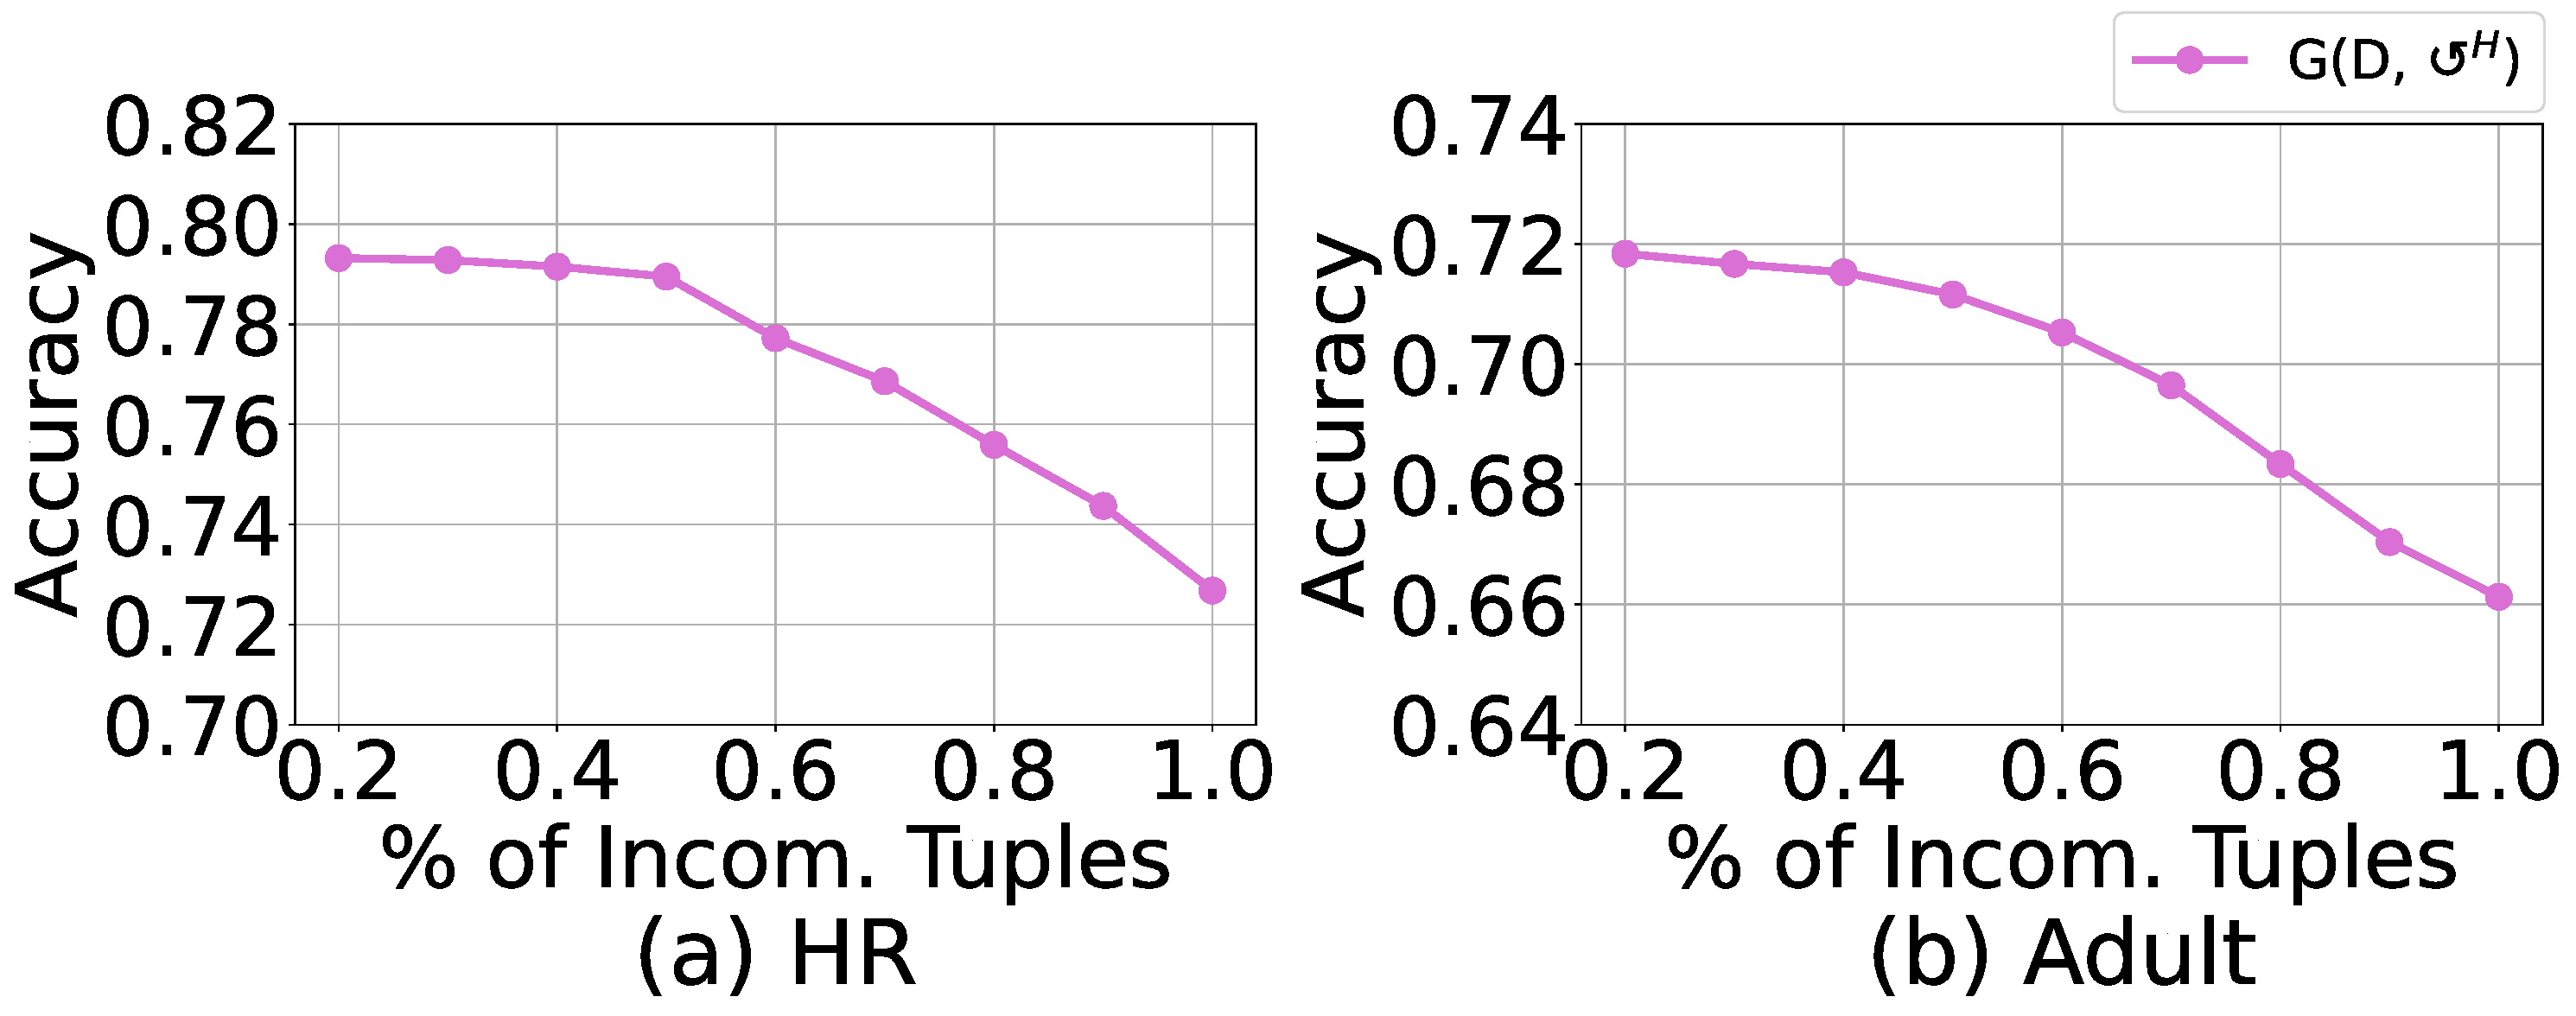
\includegraphics[width=0.7\columnwidth]{figs/missingrate_all}
%	\vspace{-1.5em}
%	\caption{Varying missing tuple rate.}
%	\label{fig:vary_misstuple_all}
%	\vspace{-1em}
%\end{figure}





%\begin{figure}
%	\centering
%	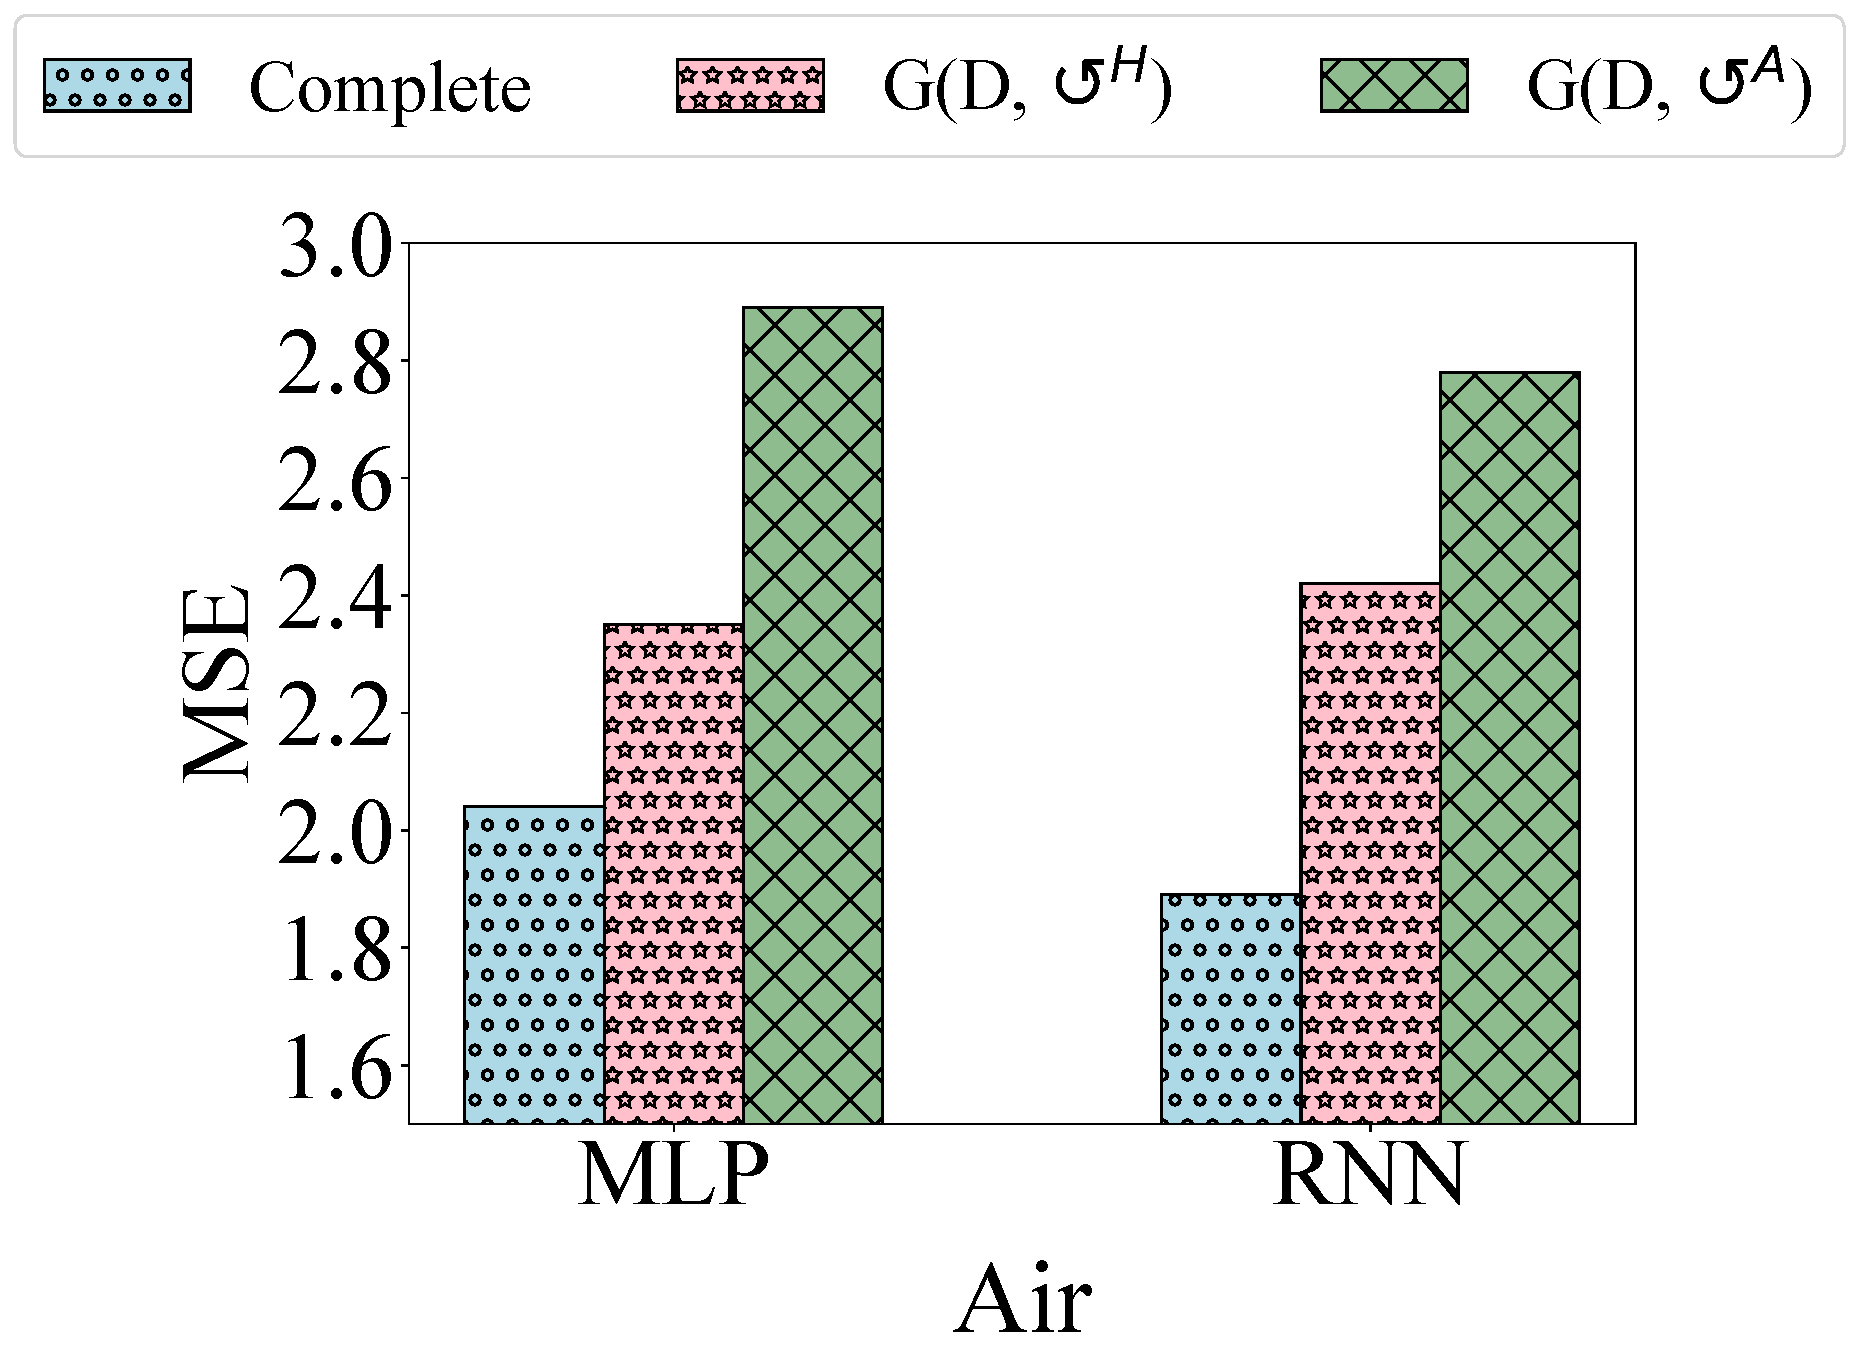
\includegraphics[width=0.5\columnwidth]{figs/downstream_fail}
%	\vspace{-1.5em}
%	\caption{Varying downsteam model (Non-convex model fails).}
%	\label{fig:downstream_fail}
%	\vspace{-2.2em}
%\end{figure}






